%! TEX program = pdflatex
\documentclass[arbeit=studie,oneside,BCOR=12mm]{ArbeitRST}
\usepackage{amsmath} 
\usepackage{afterpage}
\usepackage{placeins}
\usepackage{algorithm}
\usepackage{algpseudocode}
\hypersetup{
    unicode=false,          % non-Latin characters in Acrobat’s bookmarks
    pdftoolbar=true,        % show Acrobat’s toolbar?
    pdfmenubar=true,        % show Acrobat’s menu?
    pdffitwindow=false,     % window fit to page when opened
    pdfstartview={FitH},    % fits the width of the page to the window
    pdftitle={Verbessung der Spurerkennung und -verfolgung autonomer Modellfahrzeuge}, % title
    pdfauthor={James Vero Asghar},     % author
    pdfsubject={Subject},   % subject of the document
    pdfcreator={James Vero Asghar},   % creator of the document
    pdfproducer={Producer}, % producer of the document
    pdfkeywords={stanley controller} {sliding window method} {model cars}, % list of keywords
    pdfnewwindow=true,      % links in new window
    colorlinks=true,        % false: boxed links; true: colored links
    linkcolor=blue,         % color of internal links (change box color with linkbordercolor)
    citecolor=green,        % color of links to bibliography
    filecolor=magenta,      % color of file links
    urlcolor=cyan           % color of external links
}
\setlength{\parindent}{0ex}
\setlength{\parskip}{2ex}

% Entfernt die farbigen Markierungen - bitte Druckversion mit dieser Option kompilieren
%\hypersetup{hidelinks}

\graphicspath{{./photos}}

\addbibresource{refs.bib}
\begin{document}

% Titelseite
% ==========

% Name des Verfassers
\author{James Vero Asghar}

% Geburtsort
\geburtsort{Austin, Texas, Vereignete Staaten}

% Geburtsdatum
\geburtsdatum{3. Dezember 1997}

% Titel der Arbeit
\title{Verbesserung der Spurerkennung und -verfolgung autonomer Modellfahrzeuge}

% Untertitel
\subtitle{}

% Angabe der Betreuer
\betreuer{Dr.-Ing. Carsten Knoll}
\betreuer{M.Sc. Paul Auerbach}

% Datum der Einreichung
\date{2. Februar 2222}


% Zunächst für das Vorgeplänkel römische Seitenzahlen und einfacher Seitenstil
% ============================================================================
\pagenumbering{Roman}
\pagestyle{plain}


% Titelseite erstellen
\maketitle


% Selbstständigkeitserklärung
% ===========================

% Selbstständigkeitserklärung erstellen
\selbststaendigkeitserklaerung


% Kurzfassung / Abstract
% ======================
\kurzfassung{An dieser Stelle fügen Sie bitte eine deutsche Kurzfassung ein.}
{At the Connected Robotics Lab (CoRoLa) research group at the Barkhausen
Institut, a demonstration using remote controlled 2 axis vehicles was
developed. The demonstration is currently in use in order to model
communications between vehicles similar to an Internet of Things (IoT) network.

In order to better model the complexities of a real world system a nonlinear
control algorithm was introduced to the system in order to more accurately
control the vehicles. The Stanley Controller is a nonlinear controller
developed for use with the lateral control of 2 axis vehicles in mind. As input
to the controller, a fisheye camera was used to create images of road. These
images were then digitally processed to find the yellow line for the vehicles
to follow.}


% Inhaltsverzeichnis
% ==================
\tableofcontents

\chapter{Einleitung}

Die Forschungsgruppe Connected Robotics Lab (CoRoLa) am Barkhausen Institut hat
eine Demonstration entwickelt, die ferngesteuerte zweiachsige Fahrzeuge
verwendet, um die Kommunikation zwischen ferngesteuerten Fahrzeugen in einem
Internet of Things (IoT)-Netzwerk zu modellieren.

Aufgrund der Einschränkungen der bisherigen Fahrzeugregelung, wie z. B. der
geringen Vorwärtsgeschwindigkeit und der mangelnden Robustheit, wurde
vorgeschlagen, eine neue Regelstrategie zu implementieren. Um dieses Ziel zu
erreichen, umfasst die vorgeschlagene Lösung die Erstellung einer
Bildverarbeitungspipeline und die Implementierung des Stanley-Reglers.

\chapter{Regelalgorithmus}

\section{Stanley-Regler}

In \cite{stanley} wurde im Jahr 2005 ein Regelungsalgorithmus vorgeschlagen,
der Stanley-Regler. Von den Autoren wird dieser Regler (vermutlich unter
Bezugnahme auf die Stanford University) als "Stanley-Regler" bezeichnet.

Der Stanley-Regler ist ein nichtlinearer Regelungsalgorithmus, der 2005 von
der Stanford University entwickelt wurde, um ein zweiachsiges Fahrzeug nur
anhand der Ausrichtung des Fahrzeugs relativ zur Bahn und der Querabweichung der zu verfolgenden Bahn zu
steuern. Der Algorithmus hat sich für das kinematische Modell eines
zweiachsigen Fahrzeugs als asymptotisch global stabil erwiesen. \cite{stanley}

Der Stanley-Regler ist ein Pfadfolgeregler anstelle eines
Trajektorienfolgereglers. Als Querregler soll er das Fahrzeug auf der Bahn
halten, hat aber keinen Einfluss auf die Vorw"artsgeschwindigkeit. Dieser
Ansatz ermöglicht eine flexible Wahl der Fahrzeuggeschwindigkeit, die unter
Berücksichtigung dynamischer Effekte nach Bedarf für eine bestimmte Anwendung
gewählt werden kann. \cite{stanley}

Der Stanley-Regler wird mathematisch durch die folgende Gleichung beschrieben:
\begin{equation} 
  u = \theta - \theta_d + \arctan\left(\frac{ke_{V}}{v}\right).
  \label{eq:Stanley-Regler} 
\end{equation}
Dabei ist $u$ der Reglerausgang, welcher im Wesentlichen die "Anderung des Lenkwinkels
bestimmt, siehe \eqref{eq:model}, $\theta$ die aktuelle Ausrichtung des Fahrzeugs,
$\theta_d$ die Kursausrichtung, $k$ ein Skalierungsfaktor, $v$ die
Geschwindigkeit des Fahrzeugs und $e_{V}$ die Querabweichung vom Mittelpunkt
der Vorderachse des Fahrzeugs zum Kurs.

Der Stanley-Regler besteht aus zwei Komponenten: einer Komponente, die die
Differenz zwischen der Ausrichtung des Fahrzeugs und der des Kurses behandelt,
und einer Komponente, die die Querabweichung des Fahrzeugs vom Kurs behandelt.
Die erste Komponente, dargestellt durch $\theta_d - \theta$, steuert den
Lenkwinkel so, dass er parallel zum zu verfolgenden Kurs bleibt. Die zweite
Komponente wird durch $\arctan(\frac{ke_{V}}{v})$ dargestellt und beeinflusst
den Lenkwinkel so, dass er sich auf den Kurs zubewegt, wenn sich das Fahrzeug
weiter von ihm entfernt. Zusammen bewirken diese beiden Komponenten, dass das
Fahrzeug auf den gewünschten Kurs gelenkt wird. \cite{steering-methods}


\subsection{Kleinsignalverhalten}


Um das Verhalten des Stanley-Reglers besser zu verstehen, wird der Regler um
den Arbeitspunkt $\left(x_V, \theta_d\right) = \left(0, 0\right)$
linearisiert: 
\begin{equation} \bar{u} \approx \bar{\theta} + \frac{k}{v}e_{V}, 
    \label{eq:linearer Stanley-Regler}
\end{equation}
wobei $\bar \theta:= ... $ gilt, und die Geschwindigkeit $v$ als konstant
angenommen wird. Die sich daraus ergebende Gleichung \eqref{eq:linearer
Stanley-Regler} hat die Form eines PD-Reglers. Die P-Komponente wird durch
\(\frac{k}{v}e_{V}\) gebildet. Da die Vorwärtsgeschwindigkeit des Fahrzeugs als
konstant angenommen wird, besteht eine Proportionalität zwischen den
Ableitungen von der Querabweichung \(e_{V}\) nach Zeit und Ort. Die Ableitung
von \(e_{V}\) nach dem Ort ist \(\theta\). Daher enspricht im linearisierten
Stanley-Regler die Orientierungsdifferenz \(\bar\theta\) der D-Komponente.

\subsection{Gro{\ss}signalverhalten}

Bei großen Signalen wird der Stanley-Regler durch das Verhalten der
$\arctan$-Funktion sowie durch die zyklische Natur der Ausrichtung
\(\theta\) dominiert. Die Funktion $\arctan$ ist auf einen Wert zwischen
-90 und 90 Grad begrenzt und ist glatt. Die Ausrichtung ist ebenfalls auf den
vorderen Halbkreis des Fahrzeugsichtfelds bzw. -90 und 90 Grad begrenzt, da davon ausgegangen wird,
dass sich das Fahrzeug in eine Richtung bewegt. Zusammen begrenzen diese
Komponenten den Lenkwinkel des Fahrzeugs.

\section{Simulation}

Um ein besseres Verständnis für das Verhalten des Stanley-Reglers in einem
Modellfahrzeug zu gewinnen, habe ich eine Simulation des
Regelkreises durchgeführt. Die Simulation umfasst drei Hauptkomponenten: den
Pfad, dem das Fahrzeug folgen muss, den Stanley-Regler und das Fahrzeugmodell.
Zur Untersuchung der Zeitreihendaten des zweiachsigen Fahrzeugs in der
Simulation wurde ein Differentialgleichungslöser eingesetzt.

Der Kurs, dem das Fahrzeug folgen muss, ist eine virtuelle Darstellung der
realen Strecke, die das Fahrzeug durchfahren wird. Eine visuelle
Darstellung der Fahrbahn findet sich in Abb. \ref{fahrbahn}. In der Simulation wird der
Kurs durch die folgende kontinuierliche statische Funktion definiert:
\begin{equation} 
  (x, y, \theta) = f(t, t_f), 
\end{equation} 
wobei $t$ und $t_f$ die Eingangsparameter Zeit bzw. Simulationsdauer sind
und $(x, y, h)$ die kartesischen Koordinaten des Pfadpunkts und die
entsprechende Ausrichtung an diesem Punkt darstellt. Diese Funktion wird für
eine beliebige Anzahl von $t$-Werten diskretisiert, um eine Liste von $(x, y,
\theta)$-Werten zu erzeugen. Der Differentialgleichungslöser bezieht den
Stanley-Controller und das Fahrzeugmodell ein, um die Zeitreihen des
zweiachsigen Fahrzeugs unter Verwendung dieser Liste als Eingabe zu
analysieren.

\begin{figure}[h]
    \centering
    \includegraphics[scale=0.5]{Fahrbahn}
    \caption{Graphische Darstellung der Fahrbahn.}
    \label{fahrbahn}
\end{figure}


Das verwendete Fahrzeugmodell ist das Modell eines zweiachsiges Fahrzeug mit
gelenkter Vorderachse. Dieses Modell wird durch die folgende nichtlineare
Zustandsraumdarstellung dargestellt: 
\begin{subequations} \label{eq:model}
    \begin{align}
        \dot{x} &= v \cos(\theta) \\ 
        \dot{y} &= v \sin(\theta) \\ 
        \dot{\theta} &= \frac{v}{l}\tan(\varphi) \\
        \dot{\varphi} &= \frac{\left(\delta-u\right)}{T}. 
    \end{align}
\end{subequations}

Die Zustandskomponenten des Modells sind $x_H$, $y_H$, $\phi$ und $\theta$, wobei
$x_H$ und $y_H$ die kartesischen Koordinaten des Mittelpunkts der Hinterachse
sind und $\theta$ die Ausrichtung des Fahrzeugs ist. $\varphi$ ist der
Lenkwinkel des Fahrzeugs. Die Eingangsgrößen des Modells sind $v$ und
$\varphi$, wobei $v$ die Geschwindigkeit des Fahrzeugs und $\varphi$ der
Lenkwinkel ist. Der Lenkwinkel $\varphi$ ist selbst ein dynamisches System, das
durch eine lineare Differentialgleichung erster Ordnung mit der
konfigurierbaren Zeitkonstante $T$ dargestellt wird. Der Parameter $l$ bezeichnet der Abstand
zwischen dem Hinterradachse und dem Vorderradachse.  Das Verhalten des
Stanley-Reglers bei dynamischen Einflüssen auf den Lenkwinkel ist von großer
Bedeutung, da die globale asymptotische Stabilität des Reglers nur für das
kinematische Zweiachsmodell nachgewiesen wurde. \cite{stanley}

Da der Stanley-Regler für die Querabweichung den Mittelpunkt der Vorderachse
benötigt, muss dieser aus der Hinterachse berechnet werden. Der Mittelpunkt der
Vorderachse wird aus den Zustandskomponenten durch die folgende statische
Funktion berechnet: 
\begin{subequations}
\begin{align}
    \underline{p}_H &:= 
  \begin{bmatrix}
    x & y
  \end{bmatrix}^T \\
  \begin{bmatrix}
    x_V & y_V
  \end{bmatrix}^T
    &= \underline{p}_H + l 
  \begin{bmatrix}
    \cos(\theta + \pi/2) \\ 
    \sin(\theta + \pi/2)
  \end{bmatrix},
  \label{eq:Transformation from Rear Axle to Front Axle}
\end{align}
\end{subequations}
wobei $x_V$ und $y_V$ die kartesischen Koordinaten dieses Vorderradachsemittelpunkts sind.
Der Parameter $\underline{p}_H$ bezeichnet die Positionsvektor des Hinterradachsemittelpunkts.

Wie bereits erwähnt, besteht der Stanley-Regler aus mehreren Teilen, die
getrennt voneinander berechnet werden k"onnen. Die Ausrichtung $\theta$ ist eine
Zustandsvariable, daher ist sie unmittelbar verfügbar. Um die Querabweichung und die
Kursrichtung zu berechnen, muss der richtige Bahnpunkt gewählt werden. Der
Stanley-Regler verwendet den nächstliegenden Bahnpunkt vom
Vorderachsmittelpunkt des Fahrzeugs, um die Ausrichtung des Kurses $\theta_d$
und die aktuelle Querabweichung $e_{V}$ zu bestimmen. Für die Simulation wird
dieser bestimmt, indem der Punkt mit dem geringsten Abstand zum
Vorderachsmittelpunkt $\delta\underline{x}$ gefunden wird. An diesem Punkt wird
dann die Ausrichtung des Kurses ermittelt. Das Skalarprodukt zwischen dem
Vektor senkrecht zur Fahrzeugausrichtung $\underline{\nu}_{\perp}$ und dem Vektor
vom Pfadpunkt zur Fahrzeugvorderachse $\delta\underline{x}$ ist die
Querabweichung $e_{V}$. Zur Verdeutlichung ist in Abb. \ref{algorithm} eine visuelle
Darstellung dieser beiden Vektoren und ihres Skalarprodukts abgebildet. Die Berechnung
der wichtigen Parameter sind in folgende Gleichungen dargestellt: \\

\begin{figure}[h]
    \centering
    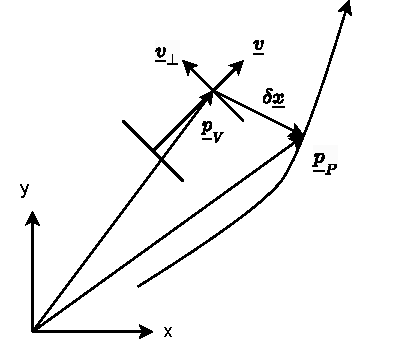
\includegraphics{dot_product}
    \caption{Grafische Darstellung der Beziehungen zwischen der ben"otigen
    Parameter. $\underline{p}_P$ ist hier der Pfadpositionsvektor mit dem
    kleinsten Abstand zum Vorderradachsemittelpunkt.}
    \label{algorithm}
\end{figure}

\begin{subequations}
\begin{align}
    \underline{\nu} &:= \begin{bmatrix} \cos(\theta) & \sin(\theta) \end{bmatrix}^T, \\
        \underline{\nu}_{\perp} &:= \begin{bmatrix} \cos(\theta + \pi/2) & \sin(\theta + \pi/2) \end{bmatrix}^T, \\
    \Delta\underline{x} &:= \underline{p}_V - \underline{p}_P, \\
    \delta\underline{x} &:= \min  || \Delta\underline{x} ||_2, \\
    \theta_d &:= \arctan\left(\frac{\frac{d}{dy}\delta\underline{x}}{\frac{d}{dx}\delta\underline{x}}\right), \\
    e_{V} &:= \delta\underline{x} \cdot \underline{v}_{\perp}.
 \label{alg:quer}
\end{align}
\end{subequations}

Der Kurs und die Querabweichung werden dann an den Stanley-Regler eingegeben,
und der Ausgang des Reglers wird in das Fahrzeugmodell eingespeist. Ein
Übersichtsdiagramm des Regelkreises ist in Abb. \ref{control_loop} dargestellt.

\begin{figure}[h]
    \centering
    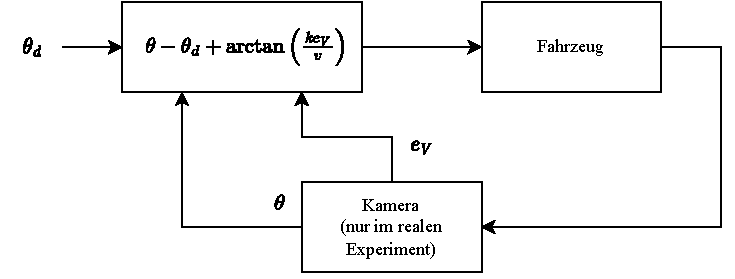
\includegraphics{control_loop}
    \caption{Darstellung des Regelkreises.}
    \label{control_loop}
\end{figure}

Der nominelle Stanley-Regler arbeitet mit zeitkontinuierlichen Signalen, die sich von den
vom \glqq echten\grqq Fahrzeug verwendeten zeitdiskreten Signalen
unterscheiden. Das Fahrzeug nimmt Bilder mit einer festen Abtastfrequenz auf,
die von der Pipeline verarbeitet werden, bevor sie in den Regler eingespeist
werden (n"aheres dazu in den Kapiteln 3 und 4). Um dieses Verhalten zu simulieren, wird ein Speicher in den Simulator
eingebaut, um die Ausrichtung und die Querabweichung zu speichern. Der
Stanley-Regler verwendet dann diese zwischengespeicherten Werte für eine
bestimmte Dauer. Dieser Speicher-Ansatz ahmt das Verhalten eines Halteglieds
nullter Ordnung nach, und die Ausgabe dieses Haltegliedes wird anschließend in
den Stanley-Regler eingespeist. Dieser Simulationsansatz ermöglicht die
Untersuchung des Fahrzeugverhaltens für verschiedene Abtastfrequenzen. Von
besonderer Bedeutung ist die Stablit"at des Regelkreises mit verschiedenen
Abtastfrequenzen. Der Vergleich der Simulationsergebnisse bei
verschiedenen Abtastfrequenzen ist in Abb. \ref{sampling} dargestellt. 

\begin{figure}[h]
    \centering
    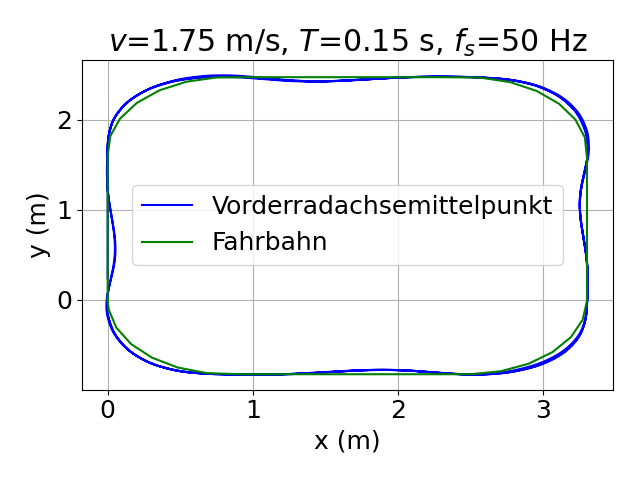
\includegraphics[scale=0.47]{50Hz}
    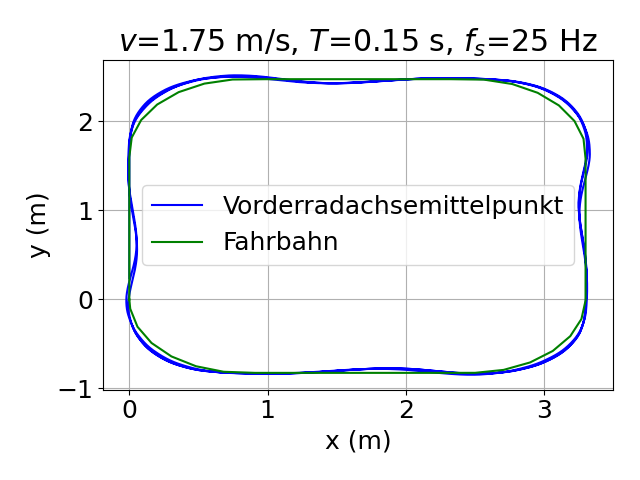
\includegraphics[scale=0.47]{25Hz}
    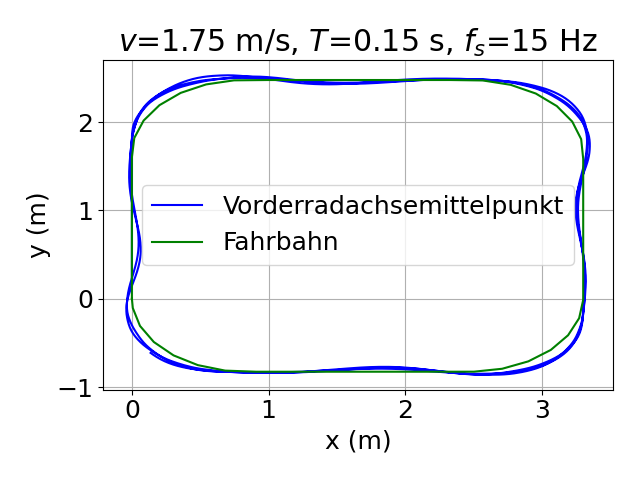
\includegraphics[scale=0.47]{15Hz}
    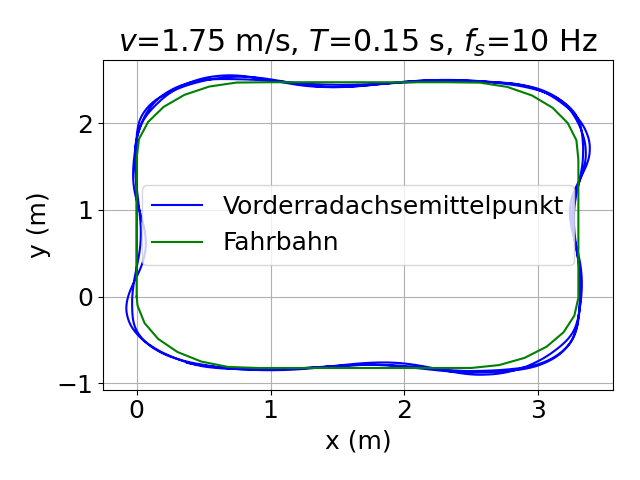
\includegraphics[scale=0.47]{10Hz}
    \caption{Verhalten des Stanley-Reglers mit verschiedenen Abtastfrequenzen.
    Das Verhalten bleibt "ahnlich bis unter 15 Hz.}
    \label{sampling}
\end{figure}

Wie in Abb. \ref{sampling} ersichtlich, wird der Stanley-Regler durch die Abtastfrequenz
beeinflusst, wobei bei niedrigeren Frequenzen ein deutlicher Effekt zu
beobachten ist. Oberhalb eines Schwellenwerts von 15 Hz scheint das
Verhalten des Fahrzeugs jedoch nicht wesentlich durch die Abtastfrequenz
beeinflusst zu werden. 

Die Simulation wurde dann für eine ausgewählte Zeitspanne durchgeführt. 



\chapter{Bildverarbeitung}
\section{Kamera-Kalibrierung}

Am Anfang der Bildverarbeitungspipeline steht die Kamerakalibrierung. Für die
CoRoLa Car Platform wurde eine Fischaugenkamera im Gegensatz zu einer
geradlinigen Kamera gewählt. Der Vorteil einer Fischaugenkamera ergibt sich aus
ihrem größeren Blickwinkel im Vergleich zu einer geradlinigen Kamera. Eine
Fischaugenkamera hat eine tonnenförmige Verzeichnung,
wodurch gerade Linien gekrümmt werden. Die Krümmung dieser Linien hängt von
ihrem radialen Abstand vom Bildmittelpunkt ab. Ein Beispiel ist in Abb.
\ref{barrel} zu sehen. Diese Verzeichnung kann mit Hilfe der Software durch die
sogenannte Kamerakalibrierung kompensiert werden. \\

\begin{figure}[h]
    \centering
    \fbox{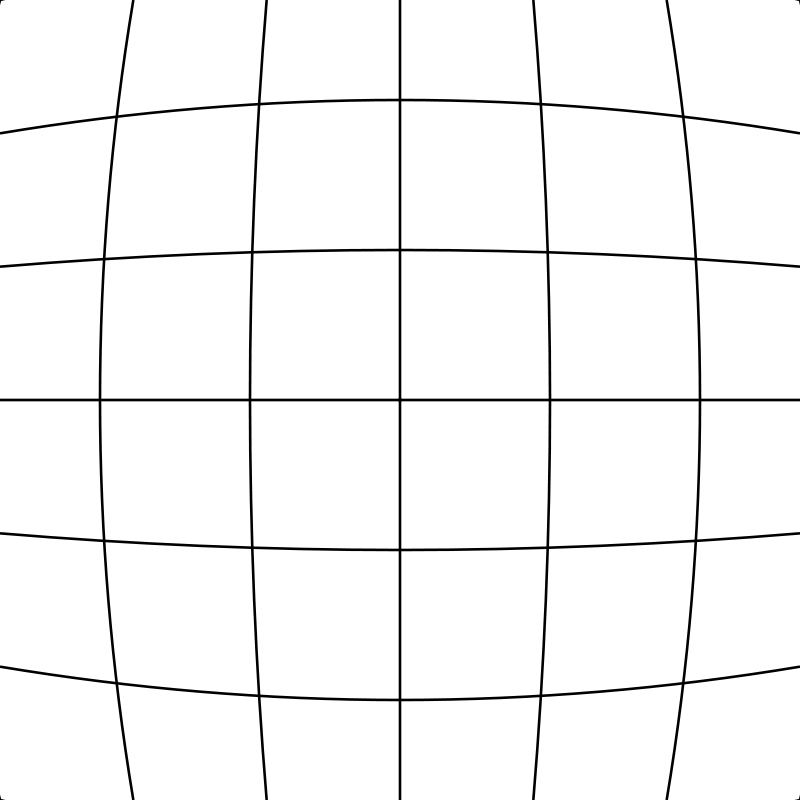
\includegraphics[scale=0.175]{Barrel_distortion}}
    \caption{Ein Beispiel einer tonnenf"ormigen Verzeichnung.}
    \label{barrel}
\end{figure}

Die Kamerakalibrierung wird verwendet, um die extrinsischen und intrinsischen
Parameter einer Kamera n"ahrungsweise zu bestimmen. Eine kalibrierte Kamera ermöglicht es,
3-D-Informationen aus einem 2-D-Bild zu gewinnen. Die intrinsischen Parameter
einer Kamera werden häufig durch die folgende 3x3-Matrix dargestellt:
\begin{equation} 
    K = 
    \begin{bmatrix} 
        f_x & 0 & c_x\\ 
        0 & f_y & c_y\\ 
        0 & 0 & 1
    \end{bmatrix}, 
\end{equation} 
wobei $f_x$ und $f_y$ die Brennweiten der Kamera in Pixeln in den
Richtungen $x$ und $y$ und $c_x$ und $c_y$ die Koordinaten des Bildmittelpunkts
sind. Die extrinsischen Parameter werden häufig durch die folgende Matrix
dargestellt: 
\begin{equation}
    \begin{bmatrix} R & T \end{bmatrix}. 
\end{equation} 
Dabei ist $R$ die Rotationsmatrix der Kamera in Bezug auf das Laborsystem (?) und $T$
der Positionsspaltenvektor des Ursprungs des Laborsystems, ausgedrückt in den
Koordinaten des Kamerabildes. Die Kameramatrix $M$ ist die Abbildung von
den Weltkoordinaten auf Pixelkoordinaten, die durch die
Matrix-Matrix-Multiplikation dargestellt wird, 
\begin{equation} 
    M = K 
    \begin{bmatrix} 
        R & T
    \end{bmatrix}. 
\end{equation} 
Durch Rekonstruieren der $M$-Matrix mit Hilfe von Software kann das verzerrte
Bild wieder in das Weltbild "uberf"uhrt werden, wodurch gekrümmte Linien gerade
werden. \\

\begin{figure}[h]
    \centering
    \fbox{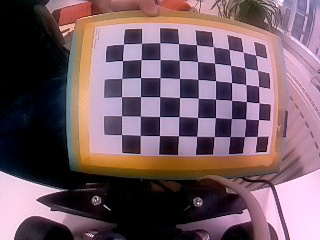
\includegraphics[scale=0.75]{before_calibration_checkerboard}}
    \fbox{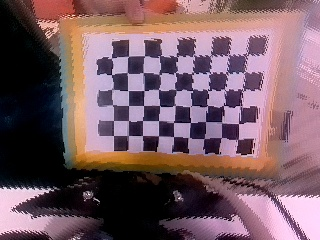
\includegraphics[scale=0.75]{after_calibration_checkerboard}}
    \caption{Die Kalibrierung des linken Bilds liefert das rechte Bild. Die gekr"ummte Linie 
    des Schachbretts sind gerade nach der Kalibrierung.} 
    \label{checkerboards}
\end{figure}

Eine Kamera wird anhand einer Sammlung von Fotos mit bekannten geraden Linien
kalibriert. In der Regel wird eine Reihe von Schachbrettbildern mit bekannten
Dimensionen verwendet. \cite{addison} Danach werden Fotos des Schachbretts in verschiedenen
Winkeln und in verschiedenen Positionen relativ zu Kamera aufgenommen. Diese Bilderserie
wird dann in den Algorithmus zur Kamerakalibrierung eingespeist, der zunächst
die Positionen der Schachbrettfelder und der sie verbindenden Linien bestimmt.
Anschließend gleicht der Algorithmus anhand des Modells einer Fischaugenkamera
die Verzeichnung aus. Wie in Abb. \ref{checkerboards} zu sehen, werden
beispielsweise die gekrümmten Linien des Schachbretts nach der Kalibrierung
wieder gerade gemacht. Die Anzahl der benötigten Bilder hängt von der
jeweiligen Kamera ab, eine große Sammlung von Fotos führt jedoch zu einer
genaueren Annäherung an die Parameter.  Die Verwendung von
Bildern mit einer höheren Auflösung führt ebenfalls zu genaueren Parametern.
\cite{addison} Die angenäherten Parameter sind jedoch nur für die
Kalibrierung von Bildern sind g"ultig, die mit der gleichen Auflösung aufgenommen
wurden wie die für die Kalibrierung verwendeten Bilder. Um die Kameramatrix für
Bilder mit einer niedrigeren Auflösung zu verwenden, muss die intrinsische
Kameramatrix $K$ mit der folgenden Formel skaliert werden: 
\begin{equation} 
    K_n = k K, 
\end{equation} 
wobei $k$ ein skalarer Wert ist, der den Skalierungsfaktor darstellt. Da es
sich bei der intrinsischen Kameramatrix um eine affine Abbildung handelt, muss
der Wert bei $K_{n3, 3}$ auf 1 gesetzt werden. Die resultierende intrinsische
Kameramatrix funktioniert bei kleineren Auflösungen, die dem Seitenverhältnis
der für die Kalibrierung verwendeten Bilder gleich sind. 


\iffalse
Allerdings wurde
beobachtet, dass bei einem zu großen Auflösungsunterschied Verzeichnungen
wieder in das Bild eingefügt werden. In ABBILDUNG ist links das Originalbild zu
sehen, das mittlere Bild wurde mit Bildern von 900p kalibriert und das rechte
Bild mit Bildern von 240p. Wie man sieht, wird das Lineal im rechten Bild
gerade, während es im mittleren Bild gekrümmt bleibt.
\fi

Ein Nachteil der Kamerakalibrierung ist, dass jedes kalibrierte Bild eine
geringere Auflösung hat als das Originalbild. Dies ist eine Folge des
Kalibrierungsprozesses, da dieser einen Teil des Bildes verzerrt,
insbesondere die Pixel in den Ecken des Bildes. Daher werden diese Pixel beim
Kalibrierungsprozess aus dem resultierenden Bild entfernt. Um das Bild in
seiner ursprünglichen Auflösung zu rekonstruieren, wird eine Interpolation
verwendet. Die Interpolation liefert jedoch ein unschärferes Bild als das
Original. Um dies zu kompensieren, empfiehlt es sich, eine Kamera mit
hochauflösenden Bildern zu kalibrieren und dann Bilder mit dieser Auflösung
aufzunehmen. Anstatt den Interpolator zu verwenden, verkleinern Sie die Bilder
dann auf eine Auflösung, die für die jeweilige Anwendung erforderlich ist.  Das
Ergebnis ist ein genaueres Bild ohne Unschärfe. Leider ist dieser Prozess sehr
rechenintensiv, und es wurde beschlossen, nur die Bilder aus dem Interpolator
zu verwenden, um die Rechenleistung der Pipeline zu erhöhen.

Ein weiterer Nachteil der Kamerakalibrierung ist, dass sich der Mittelpunkt der
Kamera verschieben kann. Ein Beispiel dafür ist in Abb. \ref{shifted} zu sehen. Durch
manuelles Ändern von $c_x$ kann der Bildmittelpunkt wieder an seine
ursprüngliche Position verschoben werden. 

\begin{figure}[h]
    \centering
    \fbox{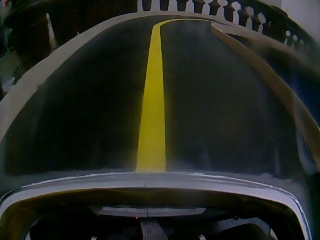
\includegraphics[scale=0.5]{orig_not_shifted}}
    \fbox{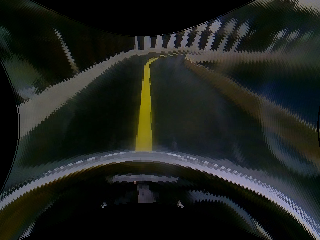
\includegraphics[scale=0.5]{cal_shifted}}
    \caption{Ein Beispiel von dem Kalibrierungsschritt. Die Mittellinie des
    rechten Bilds ist leicht nach rechts im linken Bild verschoben.}
    \label{shifted}
\end{figure}

\section{\glqq Color Thresholding\grqq}

Als Nächstes folgt der Schritt des sogenannten "Color Thresholding". In dieser
Stufe werden alle Pixel aus dem Bild entfernt, die nicht zur Bahnlinie geh"oren.
In dieser Implementierung sind Farbe ausser Gelb ungew"unscht.

Zunächst wird das Bild von allen Pixeln ohne hohen Rotanteil gefiltert, da
Hellgelb im Rot-Grün-Blau-Farbraum (RGB) einen hohen Rotanteil hat.
Anschließend wird das Bild in den HSV-Farbraum (Hue, Saturation, Value engl. f"ur Farbwert, Sättigung und
Hellwert) umgewandelt. 

Im RGB-Farbraum ist reines Gelb so definiert, dass sowohl der rote als auch der
grüne Kanal gleich sind und der blaue Kanal auf Null gesetzt ist. Dies lässt
nur einen Freiheitsgrad für die Justierung der Pipeline zu.  Ein einziger
Freiheitsgrad führt zu Problemen bei der Abstimmung, da die Pipeline dadurch
weniger in der Lage ist, Störungen zu berücksichtigen. Unterschiedliche
Lichtverhältnisse oder reflektierende Oberflächen sind Beispiele für solche
Störungen.

Im HSV-Farbraum bestimmt der Farbwertkanal die Farbe, der Sättigungskanal die
Reinheit des Farbtons und der Wertekanal die Helligkeit des Farbtons. \cite{hsv}
Nach der Auswahl des Farbwerts, in diesem Fall Gelb, werden der Helligkeits-
und der Sättigungskanal verwendet, um den spezifischen Gelbton auszuwählen. Die
Verwendung dieser beiden Kanäle ermöglicht eine zuverlässigere Erkennung der
Farbe.

Um die gelbe Spur zu erkennen, filtert die Pipeline Farben außerhalb des gelben
Farbtonbereichs heraus und schneidet dann den unteren Teil des Helligkeits- und
Sättigungskanals ab. Das Ergebnis ist, dass nur reines Gelb im Bild übrig
bleibt. Die in der Pipeline verwendeten Werte für Gelb werden durch den
folgenden Bereich, TABLE, dargestellt.

Das Ergebnis dieser Stufe der Pipeline ist beispielsweise in Abb. \ref{color-thresholding}
dargestellt. Als Eingabe bekommt der Pipeline ein kalibriertes Bild und er gibt nur Pixel aus, die 
zur Bahnlinie geh"oren. \\

\begin{figure}[h]
    \centering
    \fbox{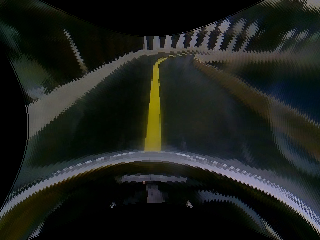
\includegraphics[scale=0.5]{calibrated}}
    \fbox{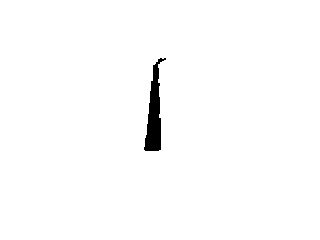
\includegraphics[scale=0.5]{thresholded}}
    \caption{Ein Beispiel von der Ausgabe des Color-Thresholdings.}
    \label{color-thresholding}
\end{figure}

\section{Perspektivtransformation}

Der dritte Teil der Bildverarbeitungspipeline ist die Perspektivtransformation. 
Das Kamera steht nicht senkrecht zur Bahn, sondern steht es winkelig zur Bahn

Wenn ein Bild mit einer am Fahrzeug montierten Kamera aufgenommen wird, ist die
Fahrbahn nicht rechteckig, sondern trapezförmig. Diese Perspektive
erfordert, dass alle Berechnungen bezüglich der Fahrspurlinie deren scheinbar abnehmende
Breite kompensieren müssen. Um dies zu vermeiden, wird eine
Perspektivtransformation durchgeführt. 

Bei der Perspektivtransformation wird eine Teilmenge eines Bildes beschnitten
und so angepasst, dass sie das gesamte Bild umfasst. Im allgemeinen Fall muss
diese Scherung nicht das gesamte Bild umfassen, sondern sie kann in einen
anderen Bildausschnitt "ubertragen werden. Ein Beispiel ist in Abb.
\ref{roi-pt} dargestellt. Bei diesem Projekt ist die Form der Teilmenge des
Bildes ein Trapez. Mithilfe dieser Perspektivtransformation wird die
trapezförmige Form der Fahrbahnlinie in eine gerade Form korrigiert, wie in
Abb. \ref{roi-pt} dargestellt. \\

\begin{figure}[h]
    \centering
    \fbox{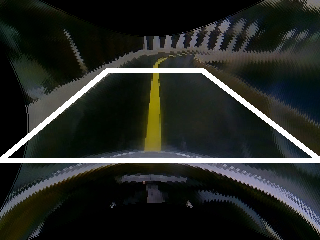
\includegraphics[scale=0.5]{roi.png}}
    \fbox{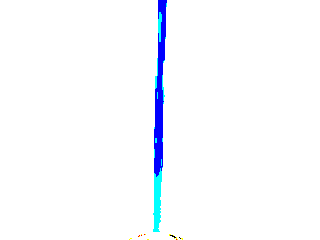
\includegraphics[scale=0.5]{perp_trans.png}}
    \caption{Ein Beispiel von der perspektivischen Transformation. Im rechten Bild ist das Trapez
    die Teilmenge, die von dem Bild beschnitten wird. (?) Im linken Bild ist die Ausgabe der
    Transformation, aber die Farbe sind invertiert.}
    \label{roi-pt}
\end{figure}

Eine Folge dieser neuen Perspektive ist, dass das resultierende Bild einer
2-D-Ebene der Strecke ähnelt. Die Perspektivtransformation vereinfacht auch die
weitere Bildverarbeitung, da alle Objekte außerhalb des Trapezes abgeschnitten
werden und nur die Spur übrig bleibt. Wie in Abb. \ref{roi-pt} zu sehen ist, führt die
Perspektivtransformation jedoch zu zusätzlichem Rauschen im Bild. Die durch die
Perspektivtransformation verursachte Scherung führt dazu, dass die Pixel des
Originalbildes gestreckt werden, wodurch das Bild mit Rauschen verunreinigt
wird. Daher ist es erforderlich, dass diese Stufe nach der
\glqq Color-Thresholding\grqq-Stufe erfolgt.

\section{Histogramm}

Nach der Perspektivtransformation wird ein Histogramm der schwarzen Pixel erstellt,
um den Startpunkt für die Gleitfenstermethode zu bestimmen. Die Anzahl der
weißen Pixel wird für jede Spalte des Bildes gezählt, und diese Zahlen werden
in einer Liste gespeichert. Es wird davon ausgegangen, dass die Spalten mit den
höchsten Zahlen Fahrspurinformationen enthalten, und der Index der Spalte mit
der höchsten Zahl wird als Startpunkt für die Gleitfenstermethode gewählt.
Dieser Schritt trägt dazu bei, die Berechnungszeit zu verkürzen, indem Teile
des Bildes herausgefiltert werden, die keine Fahrspurinformationen enthalten.
Eine visuelle Darstellung des Histogramms ist in Abb. \ref{hist} zu sehen. \\

\begin{figure}[h]
    \centering
    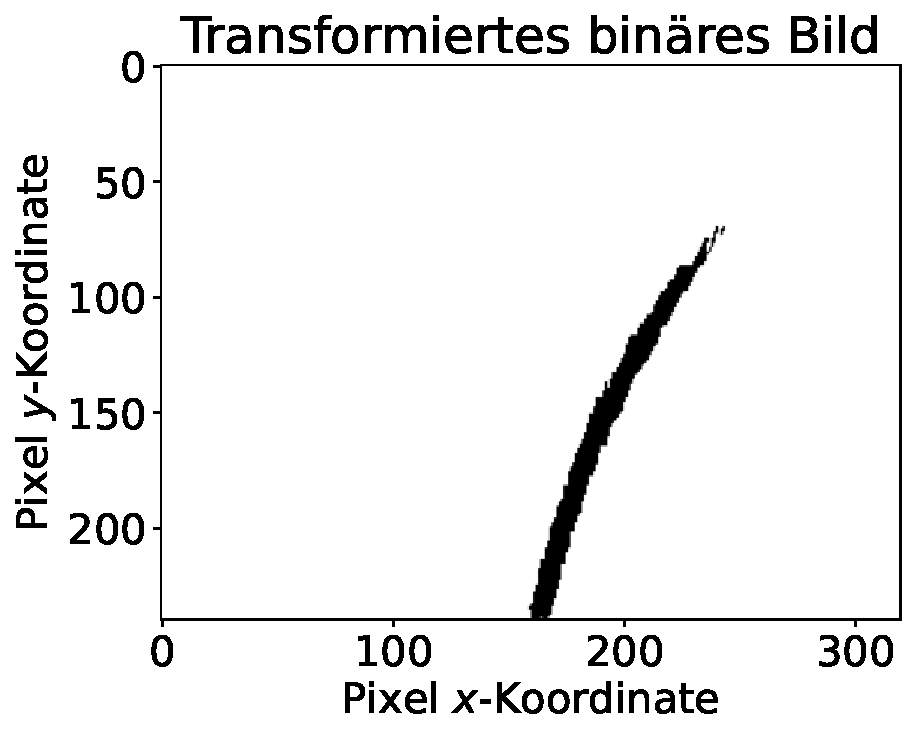
\includegraphics[scale=0.47]{hist1}
    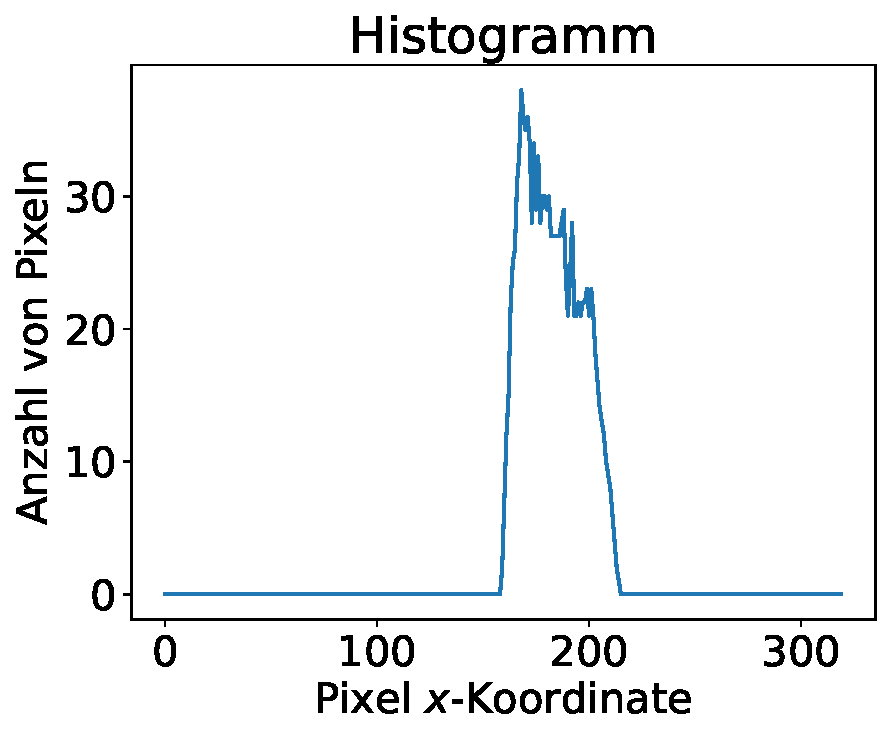
\includegraphics[scale=0.47]{hist2}
    \caption{Histogramm der schwarzen Pixel. Die Spitze des Histogramms liegt bei dem
    x-Schnittpunkts.}
    \label{hist}
\end{figure}

\section{Gleitfenstermethode}

In der fünften Stufe der Pipeline wird es erstmal die Form der Fahrspur bestimmt.

Zunächst wird eine ausgewählte Anzahl von Rechtecken (Fenstern) erstellt.  Die Höhe
wird so gewählt, dass die Summe der H"ohe aller Rechteck gleich der Bildh"ohe ist,
während ihre Breite um einen Faktor der Bildbreite gewählt wird. Die Anzahl der
Fenster wird so gewählt, dass die Spalte die schwarzen Pixel umfasst, (?) die die
Fahrspur darstellen, wie in Abb. \ref{gleit} zu sehen ist. Wenn die Anzahl der
Fenster zu groß ist, besteht die Gefahr, dass die Methode weiße Pixel, die oben 
im Bild liegen, fälschlicherweise als Teil der Fahrspur erkennt. 

Zweitens wird die x-Koordinate des Mittelpunkts des ersten Fensters auf den
Spitzenwert des Histogramms aus der vorherigen Stufe gesetzt. Dann wird die
Anzahl der weißen Pixel innerhalb des Fensters gezählt. Wenn die Anzahl über
einem gewählten Schwellenwert liegt, werden die Pixel zu einem Array
hinzugefügt und der Mittelwert der x-Koordinaten dieser Pixel
berechnet. Die x-Koordinate des nächsten Fensters wird auf diesen
berechneten Mittelwert gesetzt und um die Breite der Fenster in y-Richtung verschoben. Dieser
Vorgang wird dann für alle verbleibenden Fenster wiederholt. Wenn in einem
Fenster nicht gen"ugend schwarze Pixel enthalten sind, wird das Fenster ignoriert und das folgende
Fenster darüber gelegt.  

Die Pixel, die nicht innerhalb der einzelnen Fenster liegen, werden dann aus
dem Bild herausgefiltert. Das Bild vor und nach dem Filterungsprozess ist in
Abb. \ref{gleit} zu sehen. Mit Hilfe der Methode der kleinsten Quadrate wird ein
2. Ordnung Polynom durch die verbleibenden Pixel approximiert.

Um das Polynom, das die Fahrspur repräsentiert, aus den $n$ verbleibenden
Pixeln zu bestimmen, wird die folgende Berechnung verwendet:
\begin{gather}
    \underline{x} := \begin{bmatrix} x_1 & x_2 & ... & x_n \end{bmatrix}^T \\
    \bold{Y} := \begin{bmatrix} 1 & y_1 & y_1^2 \\ 1 & y_2 & y_2^2 \\ \vdots & \vdots & \vdots \\ 1 & y_n & y_n^2 \end{bmatrix} \\
    \underline{\hat{\beta}} := \begin{bmatrix} \hat{\beta_0} & \hat{\beta_1} & \hat{\beta_2} \end{bmatrix}^T \\
    \underline{\hat{\beta}} = \left(\bold{Y}^T\bold{Y}\right)^{-1}\bold{Y}^T\underline{x},
\end{gather}
wobei $\underline{x}$ und $\underline{y}$ die Vektoren sind, die die x- und
y-Koordinaten der übrigen Pixel enthalten. $\hat{\beta_0}$, $\hat{\beta_1}$ und
$\hat{\beta_2}$ sind die Koeffizienten des approximierten Polynoms. 

Unter Verwendung der approximierten Koeffizienten erhält man die folgende Gleichung:
\begin{equation}
    \hat{x} = \hat{\beta_0} + \hat{\beta_1}y + \hat{\beta_2}y^2,
\end{equation}
wobei $y$ die y-Koordinate und $\hat{x}$ die angenäherte x-Koordinate der
Fahrspur ist. Die Gleichung liefert eine analytische Darstellung der Fahrspur. 

\begin{figure}[h]
    \centering
    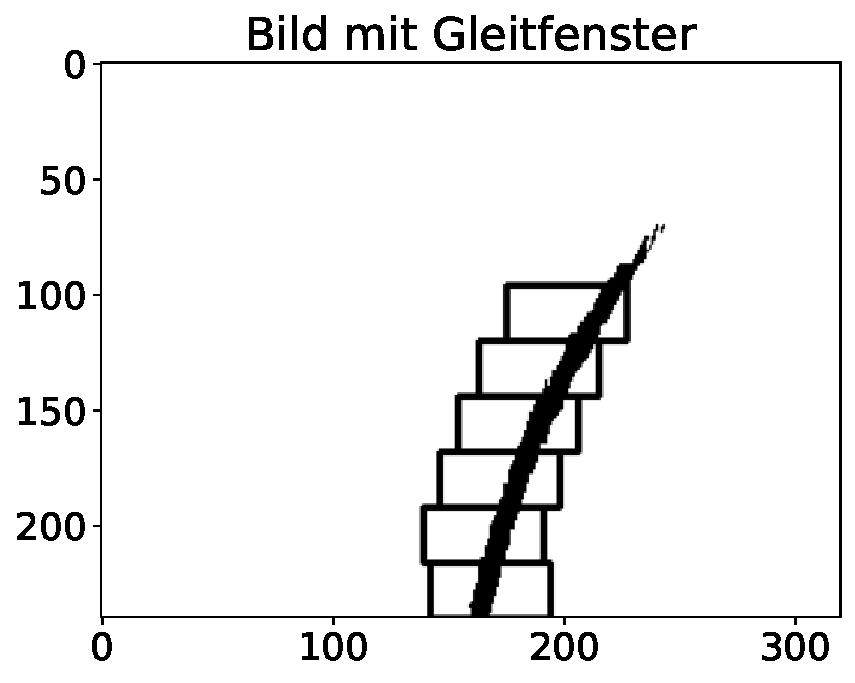
\includegraphics[scale=0.47]{before_filter}
    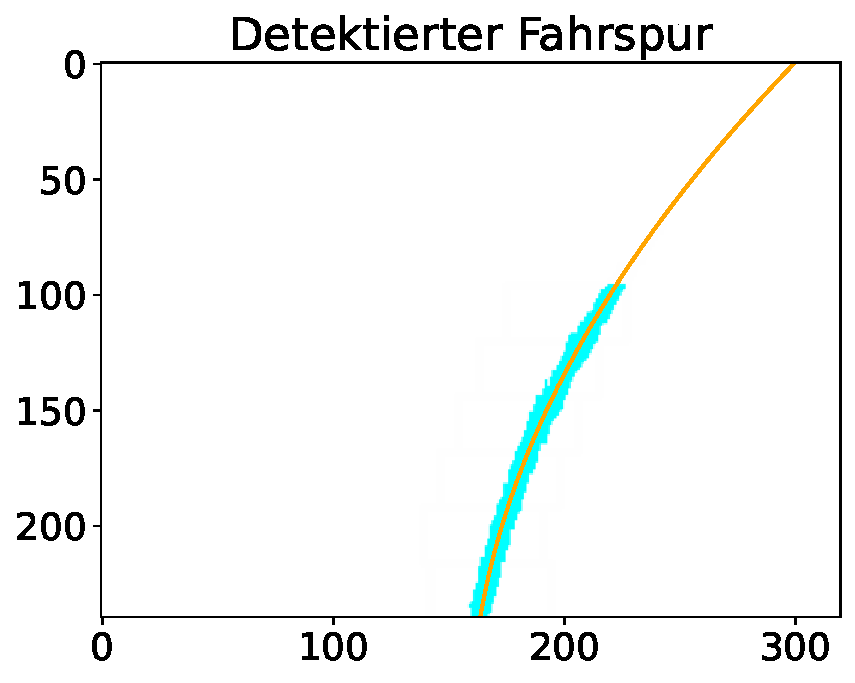
\includegraphics[scale=0.47]{after_filter}
    \caption{Das rechte Bild ist ein Beispiel von der Gleitfenstermethode. Das linke Bild
    zeigt das Polynom, das von den verbleibenden Pixel approximiert wurde.}
    \label{gleit}
\end{figure}

\section{Berechnung von Ausrichtung und Abstand}

In dem letzten Schritt der Pipeline werden die Ausrichtung des Fahrzeugs und die Abweichung von
der Fahrspurlinie berechnet. 

Aus dem in der vorangegangenen Stufe berechneten Polynom wird eine
analytische Ausrichtung an einem ausgewählten Punkt entlang der Bahn mit der
folgenden Gleichung ermittelt, 
\begin{equation} 
    \theta = \arctan(f^\prime(y)).
\end{equation} 
Der arcus Tangens der Ableitung des Polynoms liefert die
Ausrichtung der Spur an einem bestimmten Punkt. Für den Stanley-Regler wird nur die
Differenz zwischen der Bahnausrichtung und der Ausrichtung des Fahrzeugs
benötigt, da es kein globales Koordinatensystem für das Fahrzeug gibt; die
Ausrichtung des Fahrzeugs wird so gewählt, dass sie zu jeder Zeit null Grad
beträgt. In Abb. \ref{ausrichtung} ist das Koordinatensystem des Fahrzeugs
dargestellt. 

\begin{figure}[h]
    \centering
    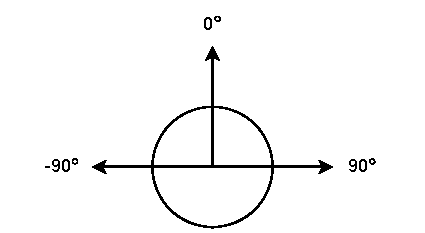
\includegraphics{fov}
    \caption{Graphische Darstellung des Modellfahrzeugsichtfelds.}
    \label{ausrichtung}
\end{figure}

\iffalse
Der klassische Stanley-Regler, wie in Kapitel 2 beschrieben, verwendet die vom
nächstgelegenen Bahnpunkt berechnete Ausrichtung. Als Nebeneffekt der
Polynomanpassung ist jedoch die am unteren Bildrand berechnete Ausrichtung
falsch. Wie in ABBILDUNG zu sehen ist, kann die Gleitfenstermethode die
Fahrspurlinie in der Nähe des unteren Bildrandes nicht konsistent erkennen. Aus
diesem Grund wird die Ausrichtung durch das angepasste Polynom falsch
approximiert. Daher wird die Ausrichtung stattdessen an einem Punkt innerhalb
der erkannten Fahrspurlinie berechnet. Außerdem wird dadurch ein zusätzlicher
Freiheitsgrad für den Regler geschaffen. Die Konsequenzen daraus werden in
Kapitel 4 erörtert.
\fi

Die Abweichung von der Fahrspurlinie wird aus dem angepassten Polynom mit
folgender Funktion berechnet: 
\begin{equation}
    e_{V} = (\frac{w}{2} - f(h))\cdot x_{mpp}.
\end{equation}
Dabei ist $w$ die Breite des Bildes, $f(h)$ die Ausgabe des berechneten
Polynoms am unteren Rand des Bildes, $x_{mpp}$ eine Skalierungskonstante zur
Umrechnung von Pixeln in Meter und $e_{V}$ der Abstand des Fahrzeugs zur
Fahrspur. Zusammenfassend wird die Differenz aus der x-Komponente des
Mittelpunkts und der x-Komponente des Polynompunkts am unteren Bildrand in
Meter umgerechnet.

\section{Ausrei{\ss}er}

Die in Algorithmen zur Fahrspurerkennung verwendete Gleitfenstermethode kann zu
einem Phänomen führen, das als \glqq Ausreißer\grqq bekannt ist. Diese treten auf, wenn
der Algorithmus die Fahrspurlinie in einem bestimmten Bild falsch bestimmt.
Abb. \ref{ausrei} zeigt eine Sequenz von drei Einzelbildern, wobei das erste linke
Einzelbild den Ausgangspunkt bildet. Im ersten Bild wird die Fahrspurlinie
richtig erkannt, aber im zweiten Bild tritt ein Ausreißer auf, bei dem die
Fahrspurlinie falsch bestimmt wird. Im letzten Bild wird die Fahrspurlinie
wieder korrekt erkannt.

\begin{figure}[h]
    \centering
    \fbox{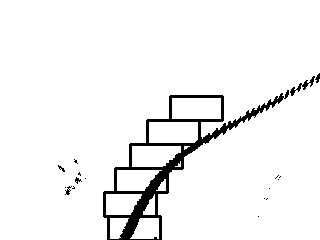
\includegraphics[scale=0.8]{before_outlier}}
    \fbox{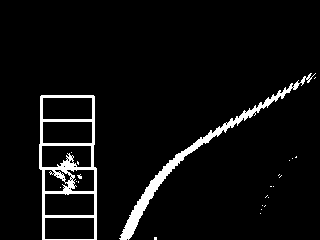
\includegraphics[scale=0.8]{outlier}}
    \fbox{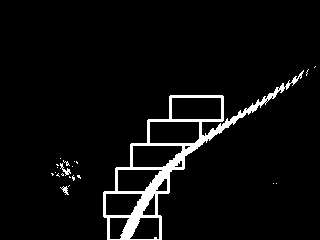
\includegraphics[scale=0.8]{after_outlier}}
    \caption{Ein Beispiel von einem Ausrei{\ss}er. Die drei Bilder sind
    nacheinander aufgenommen. Im rechten und linken Bilder sind die Fahrspur
    richtig erkannt. Im mittleren Bild ist die Fahrspur falsch erkannt.}
    \label{ausrei}
\end{figure}

Eine der Hauptursachen für Ausreißer ist die falsche Auswahl der HSV-Werte im Color-Thresholding-Schritt.
Wenn die im Algorithmus verwendeten HSV-Werte nicht restriktiv genug sind,
werden Farben außer Gelb möglicherweise nicht herausgefiltert, was zu einer
ungenauen Bestimmung der Fahrspurlinie führt.


\section{Pipeline-Optimierungen}

Bei der Entwicklung der Bildverarbeitungspipeline wurde festgestellt, dass die
Laufzeit der Pipeline zu gro{\ss} war. Um die Rechenzeit der Pipeline auf ein
akzeptables Niveau zu verbessern, wurde eine Optimierung eingeführt. Weitere
Optimierungen sind zwar möglich, würden aber den Rahmen der Arbeit sprengen und
werden daher hier nicht behandelt.

Das Python-Programm cProfiler wurde verwendet, um die Funktionsaufrufe der
Pipeline mit ihren jeweiligen Laufzeiten zu untersuchen. Da es sich bei der
Pipeline um ein deterministisches Programm handelt, verbessert die
Zwischenspeicherung der Ausgabe der teuren Funktionsaufrufe im Speicher die
Laufzeit der Pipeline. Daher wird bei allen nachfolgenden Pipeline-Ausführungen
das zwischengespeicherte Ergebnis zurückgegeben, anstatt die Berechnung erneut
auszuführen. Beispielsweise ist die Berechnung der perspektivischen
Transformationsmatrizen kostspielig, was bei der Zwischenspeicherung zu einer
Leistungssteigerung der Pipeline führt. Diese Zwischenspeicherung hat die Laufzeit 
des Pipelines vom X ms zu Y ms verringert.

Um die Leistungsverbesserung der Pipeline zu beweisen, wurde ein Experiment
durchgeführt. Zunächst wird die Pipeline einmal ausgeführt und die Laufzeit
ignoriert, da die Leistungsverbesserung nur für nachfolgende Ausführungen der
Pipeline relevant ist. Daher wird bei der zweiten Ausführung der Pipeline die
Laufzeit für beide Pipeline-Varianten gemessen, mit und ohne
Zwischenspeicherung der teuren Funktionsaufrufe aus der ersten Ausführung. Das
Experiment wird dann 100 Mal durchgeführt und das Ergebnis tabellarisch
erfasst. Das arithmetische Mittel der Laufzeiten für beide Varianten wird dann
miteinander verglichen, um die Laufzeitverbesserung zu messen. Das Experiment
zeigte, dass das Zwischenspeichern dieser Funktionsaufrufe die Laufzeit von X
ms auf Y ms senkte. (Ich muss die Werte nochmal finden.)


\chapter{Experiment}
\section{Hardware}

Die CoRoLa-Car-Platform besteht aus einem Raspberry Pi, einer Fisheye-Kamera,
einem b"urstenlosen Gleichstrommotor und einem Motorregler zur Steuerung der
Fahrzeuggeschwindigkeit und einem Servomotor um den Radeinschlag des Fahrzeugs
zu steuern. Der Raspberry Pi sendet PWM (Power-Werte) Signale an den
Motorregler und den Servoregler, um das Fahrzeug zu steuern. 

\section{Experimentkriterien}

\subsection{H"ochstgeschwindigkeit}

Um die Höchstgeschwindigkeit zu messen, fährt das Fahrzeug mit einer bestimmten
Vorwärtsgeschwindigkeit auf der Strecke. Wenn das Verhalten des Fahrzeugs als
\glqq akzeptabel\grqq angesehen wird, wird das Fahrzeug angehalten und die
Geschwindigkeit erhöht. Dieser Vorgang wird so lange wiederholt, bis das
Verhalten des Fahrzeugs nicht mehr \glqq akzeptabel\grqq ist. Das \glqq
akzeptable\grqq Verhalten des Fahrzeugs wird empirisch anhand der folgenden
beiden Kriterien definiert: Fähigkeit, der Fahrspur zu folgen, und Fehlen von
beobachteten Schwingungen.

\subsection{Maximal m"oglicher Fehlerwinkel}

Die maximalen Fehlerwinkel sind definiert als die maximalen Winkel, bei denen
das Fahrzeug in der Lage ist, den Weg links bzw. rechts der Fahrspurlinie
wiederzufinden. Um dies zu messen, wird das Fahrzeug bei deaktiviertem
Motorregler kollinear mit der Fahrspurlinie platziert. Dann wird das Fahrzeug
im Uhrzeigersinn gedreht, wobei der Ausgang des jeweiligen Reglers in Echtzeit
angezeigt wird. Das Fahrzeug wird so lange gedreht, bis der Ausgang des Reglers
entweder chaotisch wird oder konstant Null ist. Das Auftreten eines
chaotischen Ausgangs ist nicht deterministisch, empirisch gesehen ist dies
jedoch der Fall, wenn das Fahrzeug die Fahrspurlinie nicht zuverlässig erkennen
kann. Ein Ausgang von Null bedeutet auch, dass das Fahrzeug die Fahrspurlinie
überhaupt nicht erkennen kann.

\subsection{Bahnfolgeverhalten}

Die Messung des Fahrzeugversatzes erfolgt durch die folgenden zwei Versuche.
Zunächst fährt das Fahrzeug mit einer bestimmten Vorwärtsgeschwindigkeit auf
der Strecke. Dann wird mit einer Überwachungskamera ein Video von der
Kurvenfahrt des Fahrzeugs aus der Vogelperspektive aufgenommen. Das Fahrzeug
wird mit unterschiedlichen Vorwärtsgeschwindigkeiten aufgezeichnet. Bei der
ersten Aufnahmerunde wird das Fahrzeug mit dem Stanley-Regler gesteuert, bei
der zweiten mit dem PID-Regler. Dieses Experiment wird für die gewählten
Geschwindigkeiten von 1,0, 1,25, 1,5, 1,75 und 2,0 Metern pro Sekunde
durchgeführt.

\subsection{Reglerausgang}

Um den Reglerausgang der beiden Regler zu messen, wird das Fahrzeug angewiesen
(?), mindestens dreimal um die Strecke zu fahren. Während der Fahrt wird der
Ausgang des Reglers aufgenommen. Nach der Fahrt werden die Daten im Zeitverlauf
grafisch dargestellt und der Mittelwert der Daten aufgezeichnet. 

\section{Ergebnisse}

\subsection{H"ochstgeschwindigkeit}
\begin{center}
\begin{tabular}{|c|c|}
\hline
    PID & Stanley \\
\hline
\hline
    1,5 m/s & 2,3 m/s \\
\hline
\end{tabular}
\end{center}

Wenn der PID-Regler für das Modellfahrzeug verwendet wird, führen
Geschwindigkeiten von mehr als 1,5 $m/s$ zu einer geringeren Robustheit. Im
Gegensatz zum Stanley-Regler bringt der PID-Regler das Fahrzeug zum Schwingen,
wenn ein Ausreißer auftritt, und benötigt mehr Zeit, um in die Spur
zurückzukehren. Das Schwingungsverhalten nimmt mit der Vorwärtsgeschwindigkeit
des Fahrzeugs zu. Wenn die Geschwindigkeit 2,0 $m/s$ übersteigt, steuert der
PID-Regler das Fahrzeug in die Spurwand. Selbst Geschwindigkeiten zwischen 1,5
und 1,75 $m/s$ erfordern eine Überwachung, um Kollisionen zu vermeiden.

Im Vergleich dazu benötigt der Stanley-Regler keine Überwachung, bis die
Vorwärtsgeschwindigkeit des Fahrzeugs 2,3 $m/s$ erreicht. Bei höheren
Geschwindigkeiten weicht das Fahrzeug jedoch immer weiter von der gewünschten
Bahn ab, bis es sich eher wie ein Begleiter verhält als etwas, dem man folgen
muss. (?)

\subsection{Maximal m"oglicher Fehlerwinkel}
\begin{center}
\begin{tabular}{|c|c|c|}
\hline
    & PID (\textdegree) & Stanley (\textdegree)\\
\hline
\hline
    Uhrzeigersinn & 75 \pm 1& 50 \pm 1 \\
\hline
    Gegenuhrzeigersinn & 54 \pm 1 & 44 \pm 1 \\
\hline
\end{tabular}
\end{center}

Der Stanley-Regler ist im Vergleich zum PID-Regler weniger tolerant gegenüber
einer Abweichung von der Fahrspur. Dies liegt an der Kalibrierungsstufe der
Pipeline und der Anforderung eines approximierten Polynoms, was es für den
Stanley-Regler schwieriger macht, die Fahrspur zu erkennen. Im Gegensatz dazu
benötigt der PID-Regler nur eine Gruppe von gelben Pixeln im Bild.

Der Stanley-Controller benötigt für die Gruppierung der gelben Pixel eine
gewisse Geometrie, typischerweise in Form einer Linie oder eines
Kurvenabschnitts, während der PID-Controller keine solchen Voraussetzungen hat.

\subsection{Bahnfolgeverhalten}

Abb. \ref{ab:1.5}, \ref{ab:1.75} und \ref{ab:2.0} zeigen, dass der PID-Regler
die Bahn genauer verfolgt als der Stanley-Regler. Selbst unter Berücksichtigung
des anfänglichen Versatzes bringt der Stanley-Regler das Fahrzeug erst am Ende
der Kurve auf die Fahrspur, während der PID-Regler das Fahrzeug mit einer
leichten nach links driftenden Bewegung, die mit der Vorwärtsgeschwindigkeit
skaliert, auf der Bahn hält.

Die Ergebnisse der Simulation des Stanley-Reglers in Abb. \ref{sampling} mit
einer Vorwärtsgeschwindigkeit von 1,75 $m/s$ und einer Abtastfrequenz von 50 Hz
stimmen mit dem Verhalten des Stanley-Reglers auf der tatsächlichen Strecke
überein. Allerdings driftet der Stanley-Regler, wie in der Abbildung gezeigt,
vor der Kurve vom geraden Streckenabschnitt weg.

Es wurde versucht, diese Drift zu kompensieren, aber abgesehen von der
Anpassung des Bezugspunkts für die Querabweichung blieb die Drift bestehen.
Eine manuelle Änderung des Referenzpunktes führte dazu, dass das Fahrzeug bei
der Fahrt im oder gegen den Uhrzeigersinn um die Strecke unterschiedliche
Parameter benötigte, was nicht praktikabel war. Daher wurde die Drift vorerst
so belassen, wie sie ist. In Kapitel 5 werden mögliche Anpassungen des
Stanley-Reglers erörtert, die seine Leistung in Zukunft verbessern könnten.

\begin{figure}[h]
    \centering
    \fbox{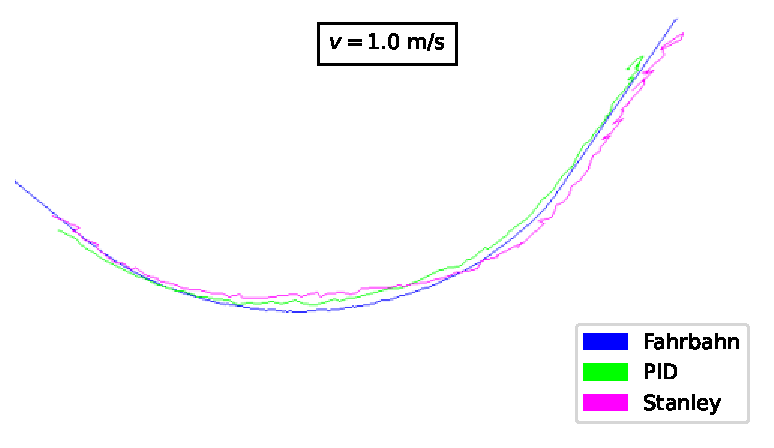
\includegraphics[scale=0.8]{done1.0}}
    \caption{PID- und Stanley-Regler haben ungef"ahr das gleiche Verhalten.}
    \label{ab:1.0}
\end{figure}

\begin{figure}[h]
    \centering
    \fbox{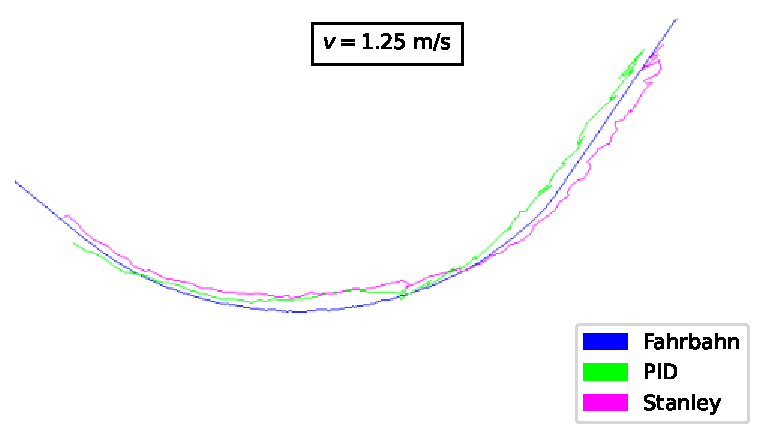
\includegraphics[scale=0.8]{done1.25}}
    \caption{PID- und Stanley-Regler haben ungef"ahr das gleiche Verhalten.}
    \label{ab:1.25}
\end{figure}
\begin{figure}[h]
    \centering
    \fbox{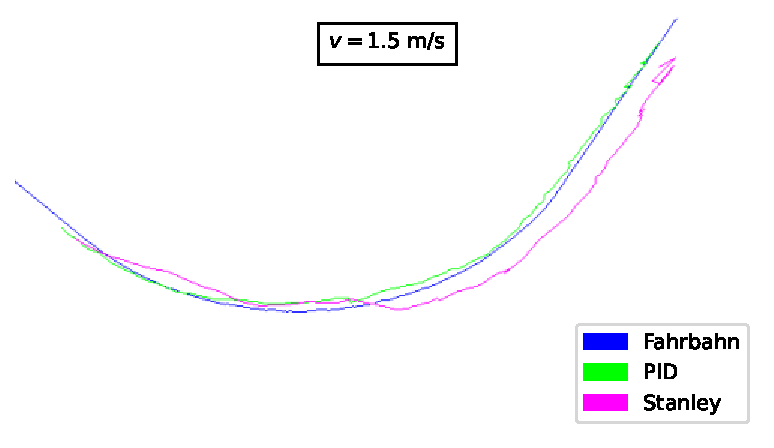
\includegraphics[scale=0.8]{done1.5}}
    \caption{Dar Modellfahrzeug mit dem Stanley-Regler hat eine kleine Abweichung am Anfang der Kurve, aber 
    am Ende der Kurve ist es nochmal auf die Fahrspur.}
    \label{ab:1.5}
\end{figure}
\begin{figure}[h]
    \centering
    \fbox{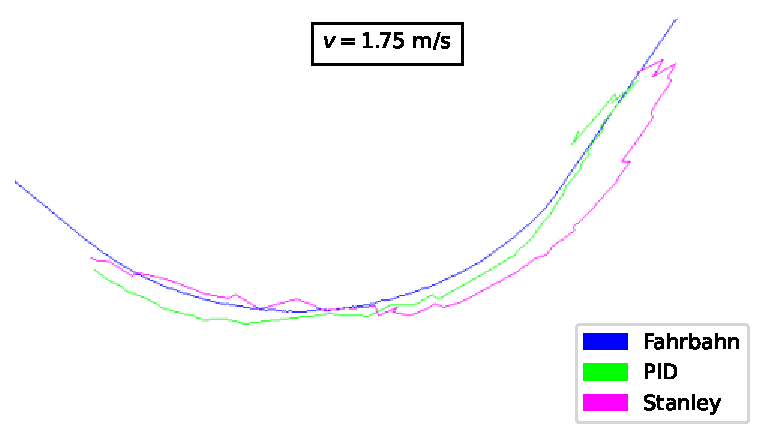
\includegraphics[scale=0.8]{done1.75}}
    \caption{Die Abweichung mit dem Stanley-Regler ist gro{\ss}er. PID-Regler verh"alt sich
    gleich.}
    \label{ab:1.75}
\end{figure}
\begin{figure}[h]
    \centering
    \fbox{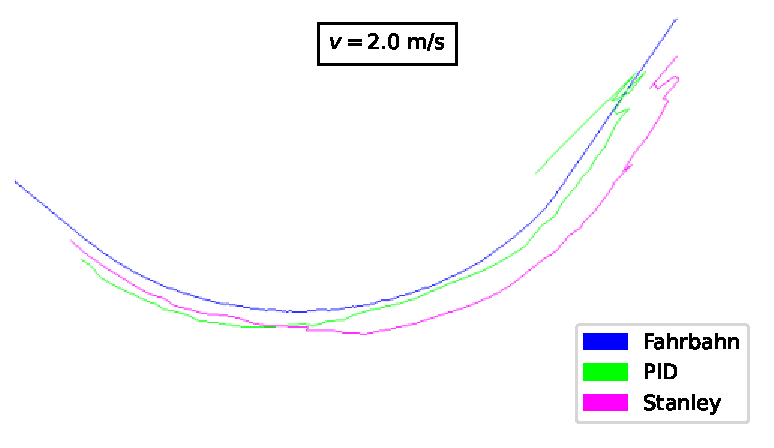
\includegraphics[scale=0.8]{done2.0}}
    \caption{Die Abweichung mit dem Stanley-Regler ist am gro{\ss}ten. PID-Regler driftet nach links
    am Ende der Kurve.}
    \label{ab:2.0}
\end{figure}
\FloatBarrier

\subsection{Reglerausgang}

\begin{center}
\begin{tabular}{|c|c|c|}
\hline
    Geschwindigkeit (m/s) & PID (\textdegree) & Stanley (\textdegree)\\
\hline
\hline
    1,0 & 5,33 & 4,79 \\ 
\hline
    1,25 & 11,97 & 11,82 \\
\hline
    1,5 & 9,61 & 13,19 \\
\hline
    1,75 & 12,35 & 13,30 \\
\hline
    2,0 & 13,84 & 13,51 \\
\hline
\end{tabular}
\end{center}

Die durchschnittliche Reglerausgabe beider Regler ist ähnlich, unabhängig von
der Geschwindigkeit, außer für den PID-Regler bei einer Geschwindigkeit von 1,5
m/s. Mit zunehmender Vorwärtsgeschwindigkeit des Fahrzeugs steigt der
durchschnittliche Reglerausgang entsprechend an. Der Unterschied zwischen den
beiden Reglern liegt jedoch in der Form der beiden Signale. Bei
Vorwärtsgeschwindigkeiten zwischen 1,0 und 1,5 $m/s$ ist der Signalverlauf der
beiden Regler ähnlich. Bei 1,75 und 2,0 $m/s$ verschlechtert sich jedoch der
sinusförmige Verlauf des PID-Reglers, während der sinusförmige Verlauf des
Stanley-Reglers zunimmt.

Bei 1,75 $m/s$ kann der PID-Regler das Fahrzeug immer noch auf die Fahrspur
lenken. Wie in Abb. \ref{reg:1.75} gezeigt, führen Ausreißer allerdings zu starken
Schwingungen im Reglerausgang. Wenn der PID-Regler die Fahrspur nicht richtig
erkennt, hat er Schwierigkeiten, das Fahrzeug auf die Fahrspur zurückzubringen.
Stattdessen kann er das Fahrzeug gegen die Wand fahren, wie am rechten Ende des
Diagramms zu sehen ist. Im Vergleich dazu hat der Stanley-Regler keine
Probleme, dem Weg mit der gleichen Geschwindigkeit zu folgen.

Bei 2,0 $m/s$ ist der PID-Regler nicht in der Lage, das Fahrzeug zu steuern, und
fährt es in die Wand. Wie in Abb. \ref{reg:2.0} dargestellt, schwankt der Ausgang
zwischen -30 und 30 Grad, und es gibt keine Periodizität. Im Vergleich dazu
weist der Stanley-Regler eine stabile Schwingung zwischen -30 und 0 Grad auf
und ist periodisch.

Ausreißer führen nicht zu starken Schwingungen, wenn das Fahrzeug mit dem
Stanley-Regler gesteuert wird. Es wurde beobachtet, dass sich das Fahrzeug viel
schneller als der PID-Regler auf der Bahn neu orientiert.

\begin{figure}[h]
    \centering
    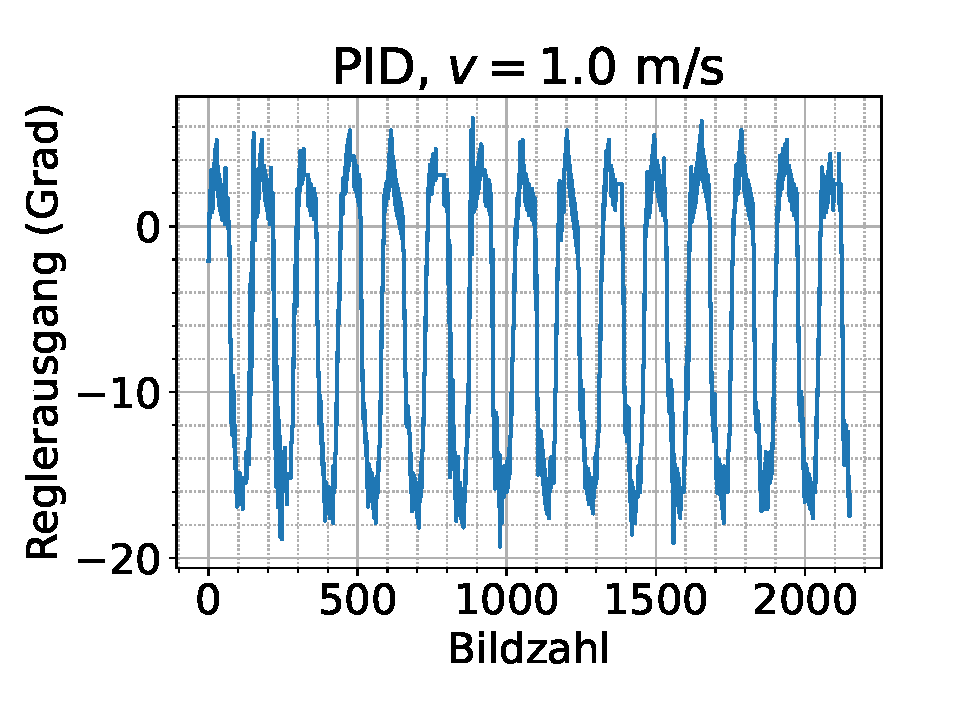
\includegraphics[scale=0.47]{pid1.0}
    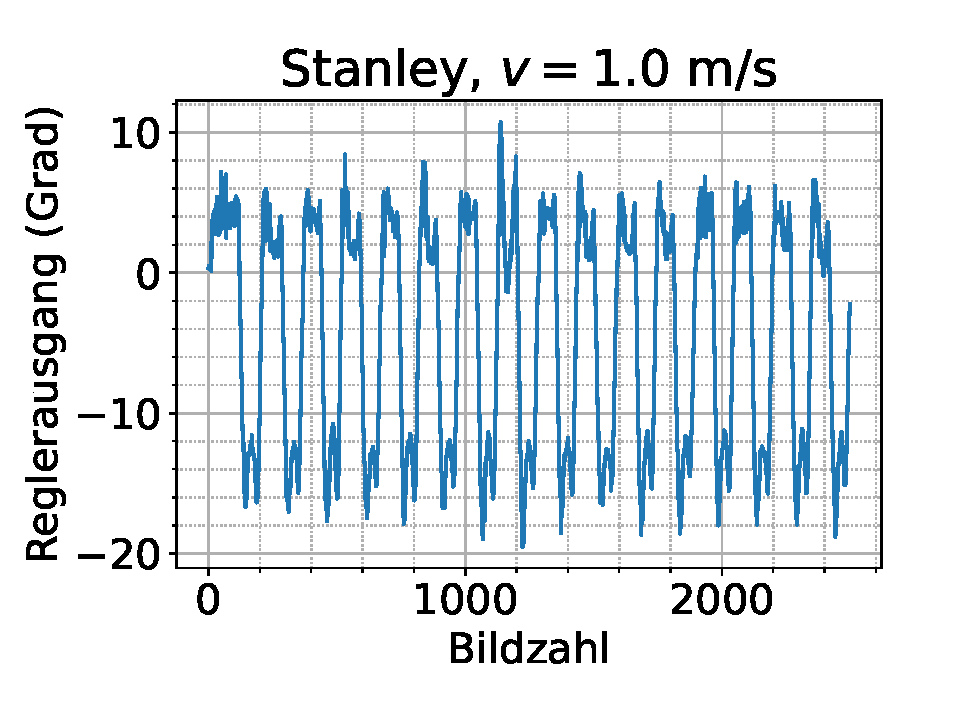
\includegraphics[scale=0.47]{Stan1.0}
    \caption{Ausgang der Regler mit $v = 1.0$ $m/s$.}
    \label{reg:1.0}
\end{figure}

\begin{figure}[h]
    \centering
    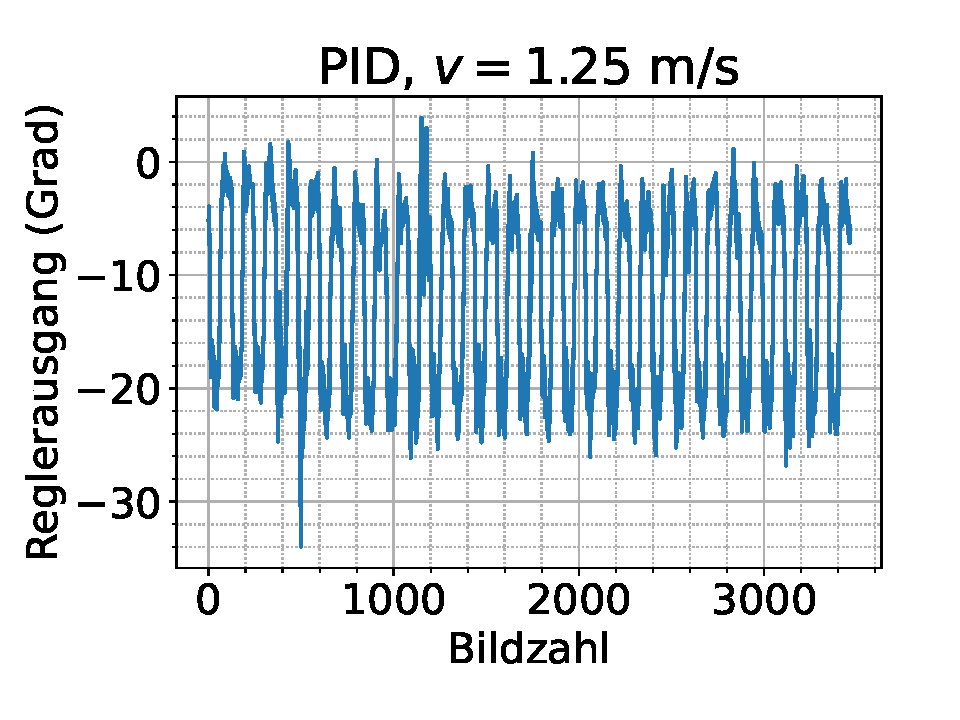
\includegraphics[scale=0.47]{pid1.25}
    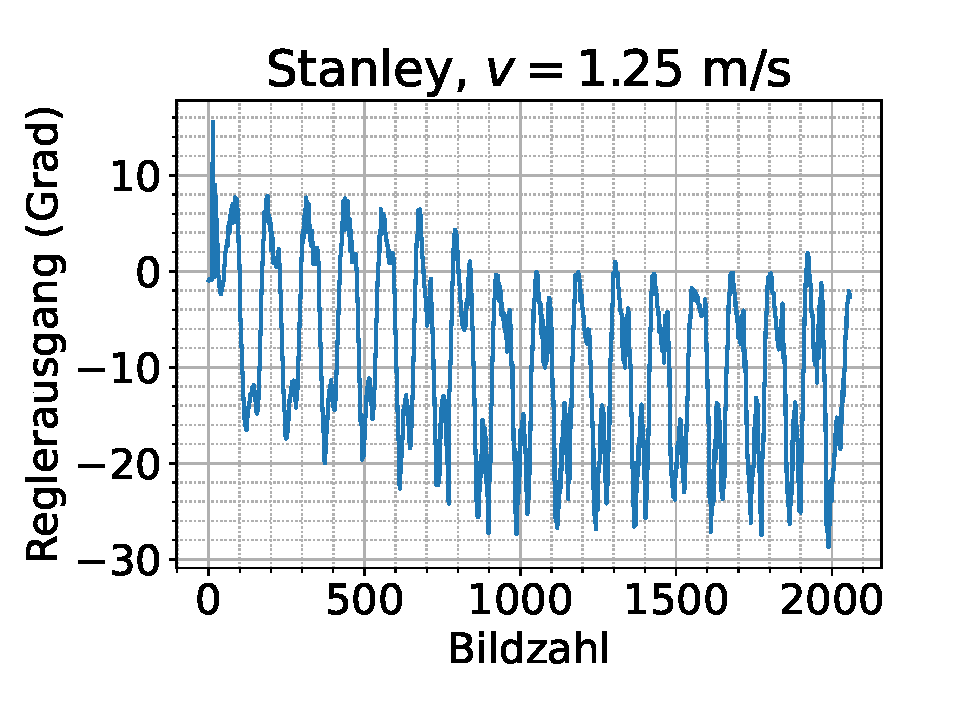
\includegraphics[scale=0.47]{Stan1.25}
    \caption{Ausgang der Regler mit $v = 1.25$ $m/s$.}
    \label{reg:1.25}
\end{figure}

\begin{figure}[h]
    \centering
    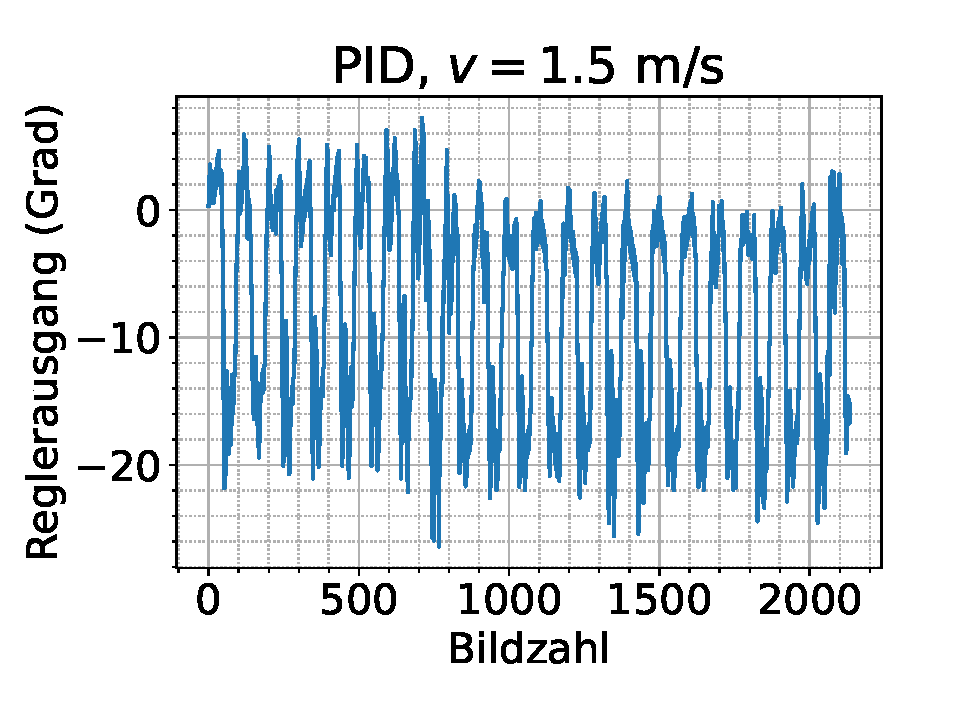
\includegraphics[scale=0.47]{pid1.5}
    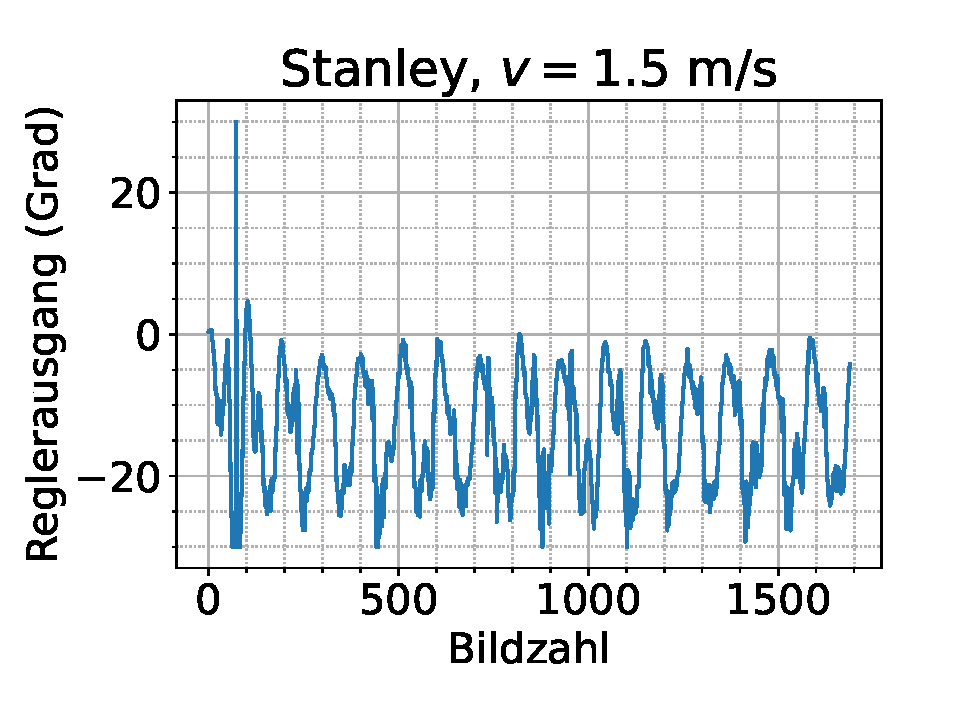
\includegraphics[scale=0.47]{Stan1.5}
    \caption{Ausgang der Regler mit $v = 1.5$ $m/s$.}
    \label{reg:1.5}
\end{figure}

\begin{figure}[h]
    \centering
    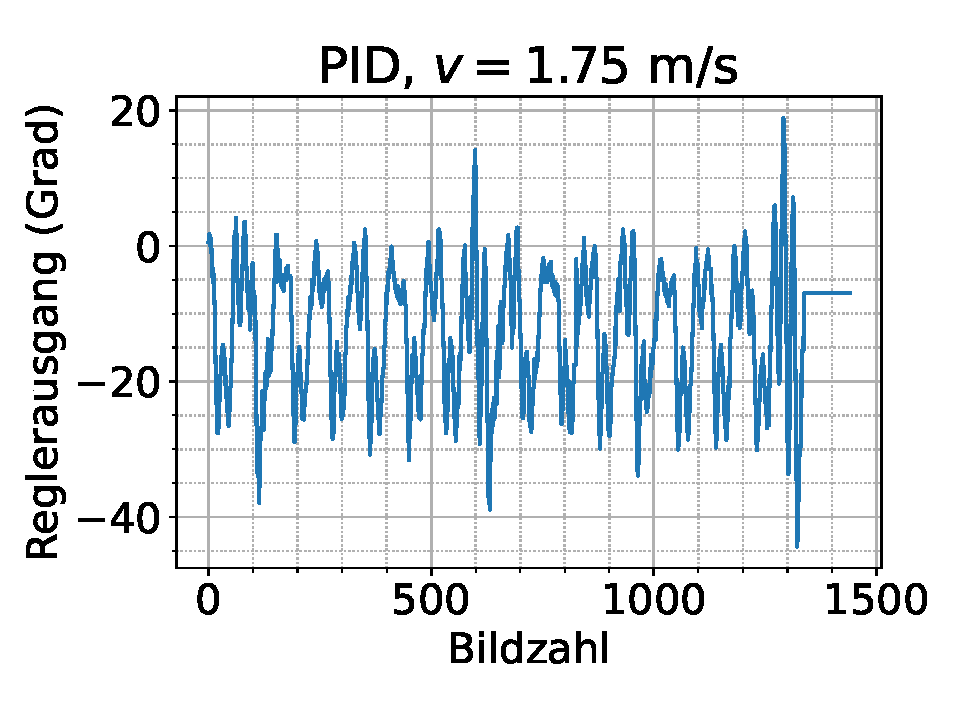
\includegraphics[scale=0.47]{pid1.75}
    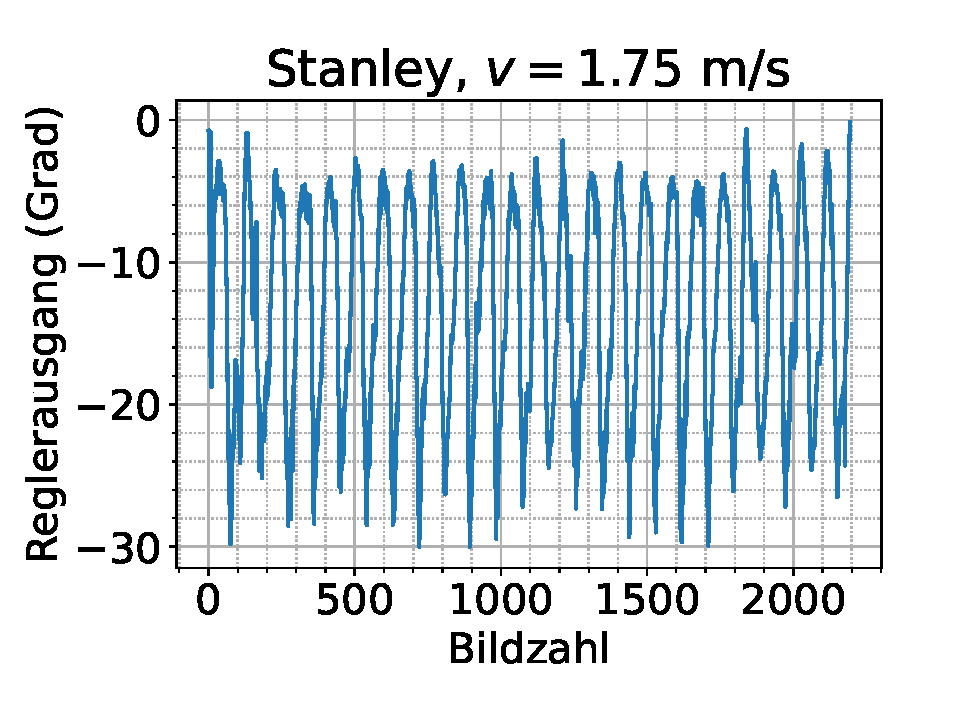
\includegraphics[scale=0.47]{Stan1.75}
    \caption{Ausgang der Regler mit $v = 1.75$ $m/s$.}
    \label{reg:1.75}
\end{figure}

\begin{figure}[h]
    \centering
    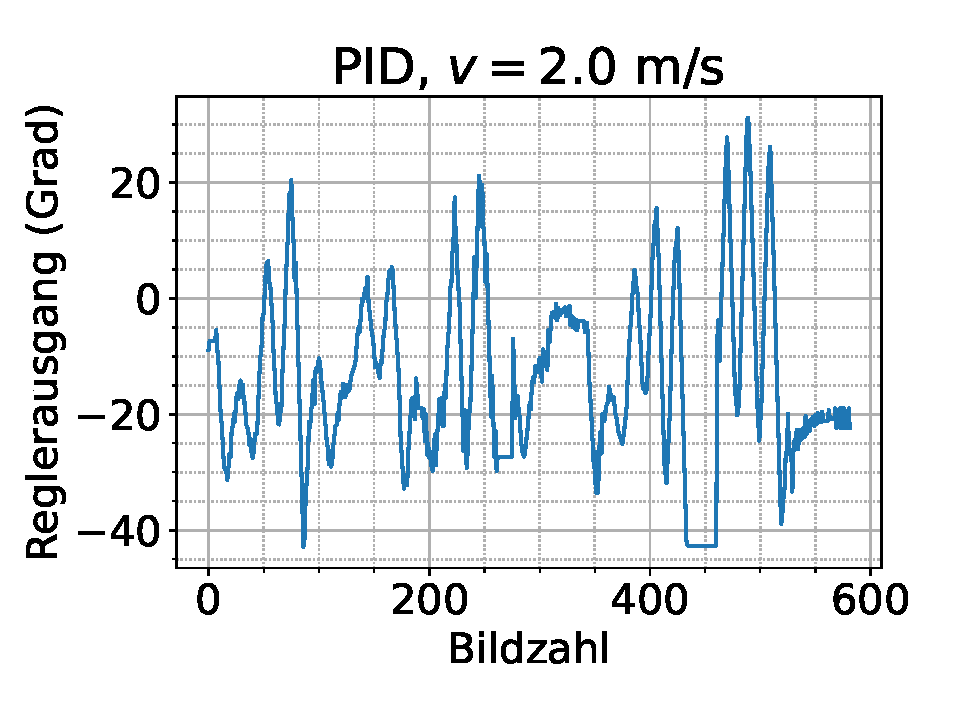
\includegraphics[scale=0.47]{pid2.0}
    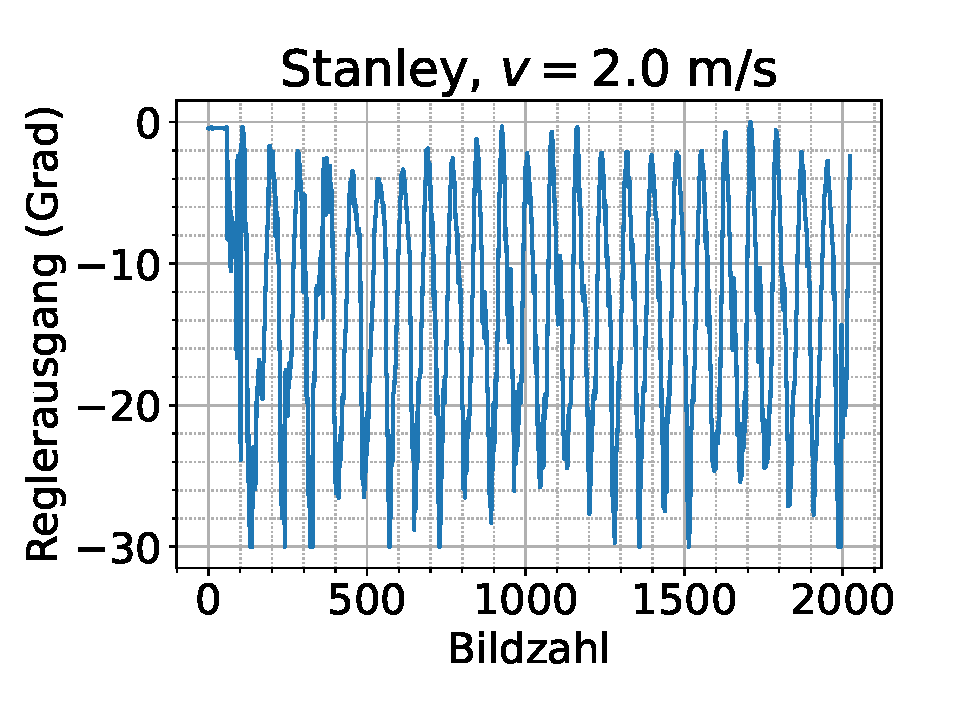
\includegraphics[scale=0.47]{Stan2.0}
    \caption{Ausgang der Regler mit $v = 2.0$ $m/s$. PID-Regler-Signal hat keine Periodizit"at
    und schwankt von -40 zu 30 Grad. }
    \label{reg:2.0}
\end{figure}




\chapter{Fazit}

Das Bahnfolgeverhalten beider Regler wurde bewertet, und während der PID-Regler
in diesem Aspekt besser abschneidet, müssen andere Faktoren der Problemstellung
berücksichtigt werden, um die bessere Lösung für die Anwendung zu finden. In
diesem Fall erweist sich der Stanley-Regler als geeigneter für die Anwendung
des autonomen Fahrens, da er in der Lage ist, höhere Geschwindigkeiten ohne
Überwachung zu bewältigen. Unter Berücksichtigung aller Aspekte der
Problemstellung ist der Stanley-Regler daher die bessere Wahl für diese
Anwendung.




\subsection{K"unfigte Arbeit}

Am Ende dieser Arbeit wurde festgestellt, dass das Fahrzeug vor jeder Kurve
immer noch von der Fahrbahn abdriftet. Um dieses Problem zu lösen, wird
vorgeschlagen, den Stanley-Regler durch Hinzufügen eines Integrators zu
verändern, um diese Abweichung zu kompensieren. Der adaptierte Stanley-Regler
wird durch die folgende Gleichung beschrieben:

\begin{equation}
    u = \theta - \theta_d + \arctan\left(\frac{ke_{V}}{v}\right) + k_{i} \int_{0}^{t} e_{V}d\tau,
    \label{eq:Stanley-Regler-adjusted}
\end{equation}

In der linearen Regelungstheorie wird ein Integrator verwendet, um bleibende
Regelabweichungen aus einer Anwendung zu entfernen. Da es sich bei der
Kleinsignalversion des Stanley-Reglers um einen PD-Regler handelt, wird
vermutet, dass das Hinzufügen eines Integrators die beobachtete Drift
korrigieren wird. Wie in der Abb. \ref{quer} zu sehen ist, ist die Drift im Eingang
des Reglers sichtbar. Durch die Integration der Querabweichung soll die Drift
mit der Zeit kompensiert werden und das Fahrzeug auf der Fahrspur bleiben.
Weitere Untersuchungen sind erforderlich, um diese Hypothese zu testen und die
Wirksamkeit der vorgeschlagenen Anpassung zu überprüfen.

\begin{figure}[h]
    \centering
    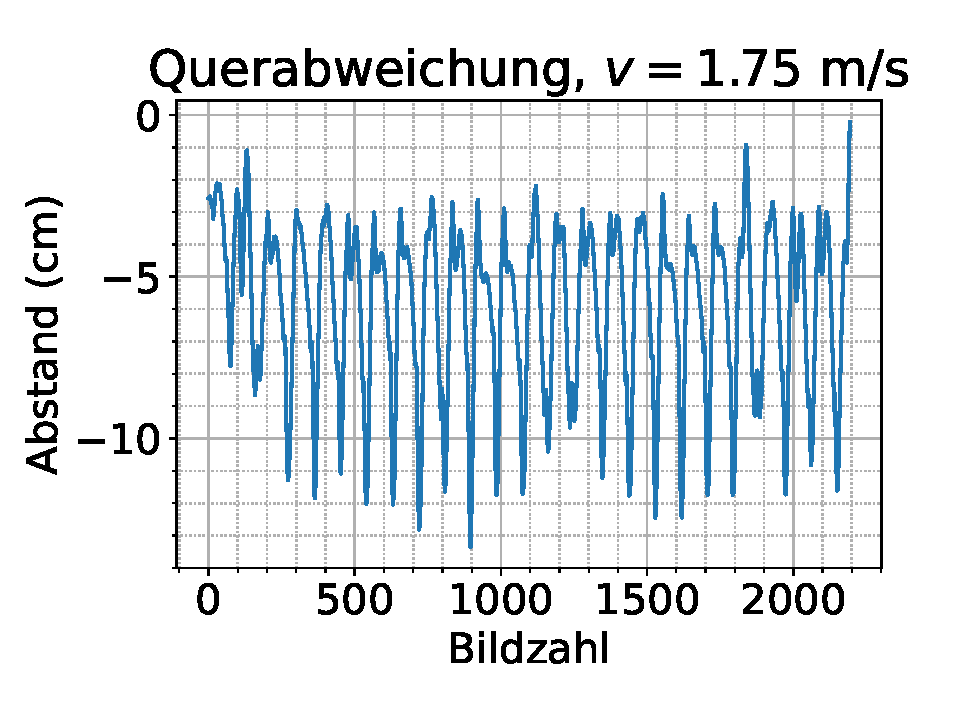
\includegraphics[scale=0.7]{querabweichung}
    \caption{Das gemessene Querabweichungsignal mit $v = 1.75$ $m/s$. Der Mittelwert
    des Signals liegt bei -5.89 cm. Deswegen gibt es ein bleibende Abweichung, die 
    mit dem urspr"unglichen Stanley-Regler nicht kompensiert wird.}
    \label{quer}
\end{figure}

\printbibliography

\end{document}
